\documentclass[12 pt]{article}
\usepackage{graphicx}
\usepackage{geometry}
\geometry{a4paper}
\geometry{margin=1in}
\usepackage{amsmath}
\usepackage{mathtools}
\usepackage{diffcoeff}
\usepackage{wrapfig}
\usepackage{hyperref}
\usepackage{titlepic}
\titlepic{
\includegraphics[width=10cm]{iitb_logo.png}}
\usepackage{pdfpages}
\hypersetup{colorlinks=true,linkcolor=blue, linktocpage}
\graphicspath{ {images/} }
\usepackage[utf8]{inputenc}

\title{\textbf{\huge DEVICE PHYSICS}}
\author{Debasish Panda 21D070021} 
\date{\parbox{\linewidth}{\centering%
  \today\endgraf\bigskip
  Mentor - Jay Sonawane \endgraf \bigskip
  \textbf{Department of Electrical Engineering}\endgraf
  \textbf{Indian Institute of Technology, Bombay}}} 

\begin{document}
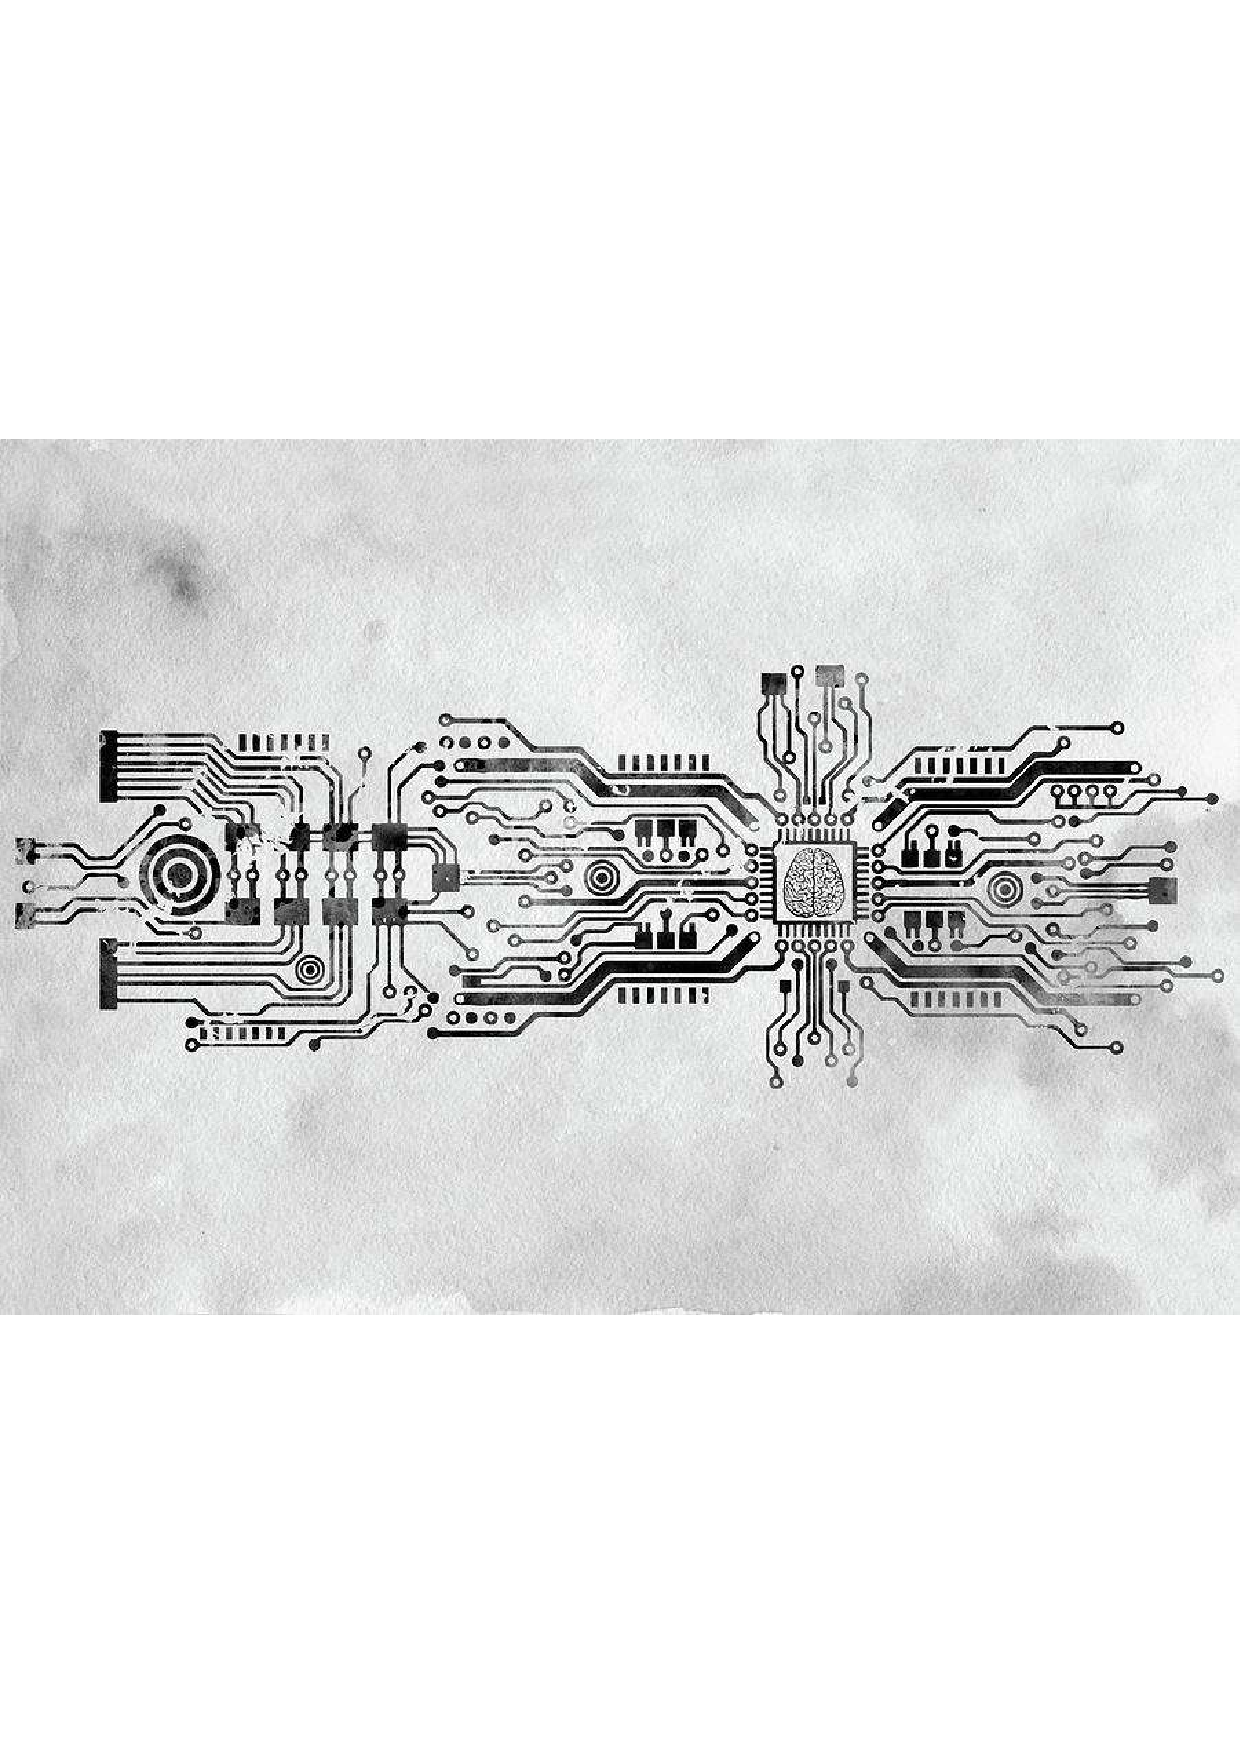
\includepdf[pages=1,fitpaper]{circuit_with_brain}

\begin{titlepage}
\maketitle
\end{titlepage}

\tableofcontents
\parskip 0.2 in
\newpage
\section{Charge Carriers in Semiconductors}

\subsection{Energy bands}
In order to fully understand the physics behind \href{https://en.wikipedia.org/wiki/Semiconductor}{semiconductors}, we need to get a clear understanding of the manner in which electrons are distributed within its crystal. Energy band diagrams serve this purpose by acting as an approximate visual guide to show how electrons are distributed in the various energy states available.  \par
Consider two carbon atoms($1s^{2}2s^{2}2p^{2}$)initially separated by a large distance from each other. In such a state, the electrons in the atoms occupy discrete,well-defined energy levels. However, as the two atoms come closer, this view no longer holds true. At a finite distance(comparable to atomic sizes) between the two atoms, their wavefunctions overlap strongly and the discrete energy states change into a near-continuum energy state distribution. As more and more atoms get involved in the crystal, the overlapping of their wavefunctions ultimately leads to the formation of 'energy bands', that are composed of numerous discrete energy levels but appear as a continuous band due to the large number of atoms involved.\newline

\par
 \begin{center}
    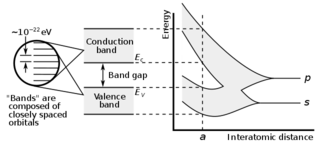
\includegraphics{energy_band_structure_1_50.png}
    \end{center}
    \begin{center}
      \emph{\hspace{0.6cm}Energy band structure in a crystal of carbon atoms}
  \end{center}
  
  \par
   \begin{center}
   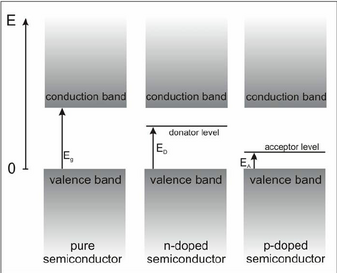
\includegraphics{ebd_1_50.png}
   \end{center}
    \begin{center}
      \emph{ Energy band diagram in semiconductors}
  \end{center}
\par
 When electrons are excited to the empty energy level, they can freely move about under external influence, and hence, conduct electricity. This band is therefore known as the conduction band. The energy band gap for semiconductors is intermediate between that of conductors and insulators-which explains their nomenclature.
\par
The energy band gaps for some of the common semiconductors are: Si-1.1 eV, Ge-0.7 eV, GaAs-1.42 eV, etc. At room temperature of around 300 K, the kinetic energy of an electron is of the order of $k_{B}T$, where $k_{B}$ represents the Boltzmann's constant. On calculating, this value turns out to be around 26 meV, far too less for an electron to be excited to the conduction band from the valence band as per the rules of classical physics. However, on the atomic scales, where the rules of quantum mechanics dominate, there is still a non-zero probability for the electron to be excited from the valence band to the conduction band. 

\subsubsection{Physical model of Semiconductor lattice}
Even though it may theoretically seem quite difficult to analyse the motion of an electron in the semiconductor lattice using quantum mechanics, it actually turns out that relatively simple physical models can appropriately describe the electron's motion to high degree of accuracy and serve nearly all our practical purposes.\par
Let us consider a free electron moving along the x-axis. The motion of the electron can be described by an E-k diagram which plots energy of the electron as a function of its wave-vector,k (The relation is established using De-broglie's hypothesis).
\begin{center}
    E = $\hbar^{2}k^{2}$/2$m_{e}$
\end{center}
where $m_{e}$ represents the rest mass of electron.\newline

  \par
  \begin{center}
   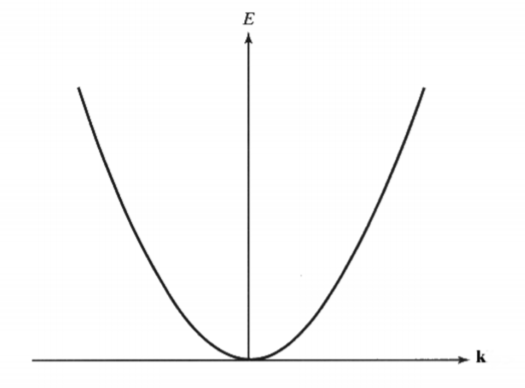
\includegraphics{1BRam.png}
   \end{center}
    \begin{center}
      \emph{E-k diagram for a free electron}
  \end{center}

\par 
However, as we can see, inside a semiconductor lattice, the assumption of a free electron no longer holds true. The electron in a crystalline lattice can be thought of as experiencing a periodic potential because of the regular, organised arrangement of atoms. As of now, we will consider the 1-D case for simplicity and the 3-D case follows as a natural extension of our analysis. \par
The 1-D crystalline lattice can be imagined of being composed of a series of Dirac-delta potential wells, each centered at one of the atoms in the lattice and at a constant distance from each other, known as the lattice constant. Now, having established a feasible model for the lattice, we can solve for the wavefunction of electron inside this 1-D lattice using \href{https://en.wikipedia.org/wiki/Bloch%27s_theorem} {Bloch's Theorem}. This 
model of particle trapped inside a one-dimensional lattice is also known as the \href{https://en.wikipedia.org/wiki/Electronic_band_structure}{Kronig-Penney model}. 

\par
\begin{center}
   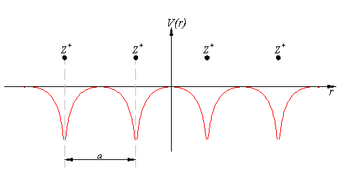
\includegraphics{Potential-actual_2_70.png}
    \end{center}
    \begin{center}
      \emph{Periodic potential inside the crystal lattice}
  \end{center}
\par

  \par
  \begin{center}
   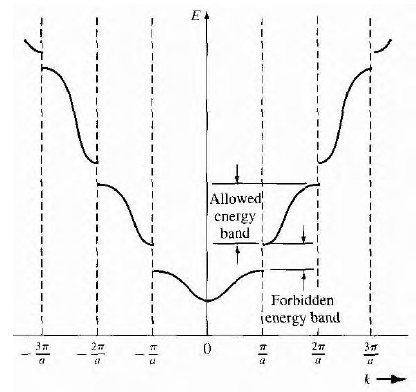
\includegraphics{93mtK.png}
    \end{center}
    \begin{center}
      \emph{E-k diagram for an electron inside the lattice}
  \end{center}
\par

As we can observe, there are several discontinuities in the graph at quantized values of k. However, for most of the practical semiconductor devices, the majority of electrons lie in the range of $-\pi/a < k < \pi/a$, otherwise known as the first Brillouine zone. In this region, we can approximate the graph to be parabolic in nature and express effective mass($m^{*}$) of the electron as:

\begin{center}
    $m^{*}$ = $\hbar^{2}/\frac{\partial^2 E}{\partial k^2}$
\end{center}


\subsubsection{Concept of holes}

When an electron is excited from the valence band to the conduction band, it leaves behind an "empty space" in the energy state it previously occupied. In such a situation, when an external electric field is applied, the electron adjacent to the hole moves forward to fill the empty slot. This process continues and thus creates an electric current due to the net motion of the electrons. Physically, this is equivalent to a positive charge of the same magnitude as the electronic charge, constituting a current. Such a quasi-particle has been assigned the name 'holes' and constitute another type of the charge carriers found in a semiconductor.


\subsection{Carrier Statistics}

Electrons and holes are fermions- meaning they have half-odd-integer spin and follow \href{https://en.wikipedia.org/wiki/Pauli_exclusion_principle}{Pauli's exclusion principle} . The statistical rules governing the dynamics of an ensemble of such fermions are known as the \href{https://en.wikipedia.org/wiki/Fermi%E2%80%93Dirac_statistics#:~:text=Fermi%2DDirac%20statistics%20is%20a,of%20particles%20over%20energy%20states.}{Fermi-Dirac statistics}.

\subsubsection{Fermi-Dirac Statistics}
The probability distribution governing Fermi-Dirac statistics is derived by using the fact that multiplicity of the system should be maximized. On doing this, we obtain the probability distribution(as a function of energy) as:
\begin{center}
    f($E_{i}$) = $(1+exp(E_{i}-E_{F}/k_{B}T))^{-1}$
\end{center}
where $E_{F}$ represents the Fermi energy level. 

  \par
  \begin{center}
   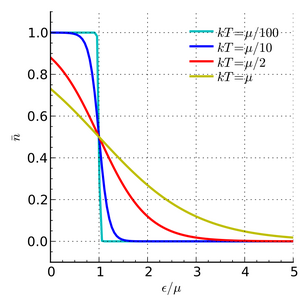
\includegraphics{1027px-FD_e_mu.svg_2_30.png}
   \end{center}
    \begin{center}
      \emph{Probability distribution graph of F-D statistics}
  \end{center}
\par

In order to estimate the number of particles occupying a given energy state, we also need to estimate the density of states function, g(E) which represents the \href{https://en.wikipedia.org/wiki/Degenerate_energy_levels}{degeneracy} of a particular energy level. The density of states functions for the C.B. and V.B. of semiconductors is as follows:
\begin{center}
    g(E) = $\frac{4\pi}{h^{3}}(2m_{e}^{*})^{3/2}\sqrt{E-E_{c}}$, for C.B.
\end{center}

\begin{center}
    g(E) = $\frac{4\pi}{h^{3}}(2m_{h}^{*})^{3/2}\sqrt{E_{v}-E}$, for V.B.
\end{center}
where $m^{*}$ and $m_{h}^{*}$ represent the effective masses of the electron and hole, respectively.

\subsubsection{Carrier concentrations}
Having obtained the density of states function and probability distribution function, we can easily obtain the total number of electrons and holes in the C.B. and V.B., respectively. The corresponding equations are given as:
\begin{center}
    $n_{e} =  \int_{E_{c}}^{\infty} g(E)f(E) \,dE \ $
\end{center}

\begin{center}
    $n_{h} =  \int_{-\infty}^{E_{v}} g(E)f(E) \,dE \ $
\end{center}

These integrals are of the form of \href{https://en.wikipedia.org/wiki/Complete_Fermi%E2%80%93Dirac_integral}{Fermi-Dirac integrals} of $1/2$ order and are expressed as:
\begin{center}
    $n_{e} = N_{c}F_{1/2}(\frac{E_{F}-E_{c}}{k_{B}T})  $
\end{center}

\begin{center}
    $n_{h} = N_{v}F_{1/2}(\frac{E_{v}-E_{F}}{k_{B}T})  $
\end{center}
where $N_{c}$ and $N_{v}$ are known as the effective conduction band density of states and $F_{1/2}$(x) represents the Fermi integral of order 1/2. Their formulae are given as follows:
\begin{center}
    $N_{c} = 2(\frac{2\pi m_{e}^{*} k_{B}T}{h^{2}})^{3/2}$
\end{center}

\begin{center}
    $N_{v} = 2(\frac{2\pi m_{h}^{*} k_{B}T}{h^{2}})^{3/2}$
\end{center}
Physically, these quantities represent the number of electrons just at the edge of the valence band or conduction band.\par

At equilibrium, if no external impurities have been added to the semiconductor lattice, it is known as an intrinsic semiconductor and in such cases, $n_{e}$ and $n_{h}$ are both equal to $n_{i}$, termed as the intrinsic carrier concentration. In a semiconductor, $n_{i}$ represents the minimum number of charge carriers that are present in it without any sort of external influence.\par

In order to get an estimate of the value of $n_{i}$, certain approximation methods can be used to evaluate the Fermi-Dirac integral associated with $n_{e}$ and $n_{h}$. If $E_{c}-E_{F} \ge 3k_{B}T$ or $E_{F}-E{v} \ge 3k_{B}T$, we can approximate the integrals as:
\begin{center}
 $F_{1/2}(\frac{E_{F}-E_{c}}{k_{B}T}) \approx exp(\frac{E_{F}-E_{c}}{k_{B}T}) $
\end{center}

\begin{center}
  $F_{1/2}(\frac{E_{v}-E_{F}}{k_{B}T}) \approx exp(\frac{E_{v}-E_{F}}{k_{B}T})$ 
\end{center}

For an intrinsic semiconductor, the Fermi energy level ideally coincides with the intrinsic energy level $E_{i} = \frac{E_{v}+E_{c}}{2}$ and the value of $E_{G}$ is considerably larger than $3k_{B}T$. So the above approximation holds true for quite a large number of the commonly used semiconductor materials. Hence, to find $n_{i}$, approximate the expression as:
\begin{center}
    $ n_{e} \approx N_{c}exp(\frac{E_{F}-E_{c}}{k_{B}T})  $
\end{center}

\begin{center}
     $ n_{h} \approx N_{v}exp(\frac{E_{v}-E_{F}}{k_{B}T})  $   
\end{center}

On multiplying the two expressions, one can observe that:
\begin{center}
    $np = n_{i}^{2} = \sqrt{N_{c}N_{v}}exp(\frac{-E_{G}}{k_{B}T})  $
\end{center}
This is one of the most important relations governing carrier concentrations in semiconductor physics.


\subsection{Doping of Semiconductors}

As we know, one of the most striking features of semiconductors is their ability to change their conductivities over a wide range of orders of magnitudes. This is achieved by \href{https://en.wikipedia.org/wiki/Doping_(semiconductor)#:~:text=In%20semiconductor%20production%2C%20doping%20is,to%20as%20an%20extrinsic%20semiconductor.}{doping of semiconductors}. Doping essentially involves addition of extraneous impurities into the semiconductor lattice which infuse the lattice with a particular kind of charge carrier and thus, decrease the concentration of the other. \par

Let us consider an example of n-type doping where phosphorus(P) atoms are added to a crystalline lattice of silicon(Si) atoms. Since P has one extra electron in its valence band as compared to Si, this electron cannot be accomodated under covalent bonding phenomena. Hence, the effective nuclear attraction experienced by the extra electron decreases and it now has a high probability of being excited into the conduction band through thermal excitation. This entire process effectively creates a positively charged, immobile ion centre at the site of the P-atom. The same goes for an electron-deficient material such as boron(B) added to the semiconductor lattice- except that this generates a hole instead of an electron. Through doping, one can reduce the concentration of minority charge carriers drastically. Consider a sample of Si crystal which is n-type doped using P atoms such that $N_{D} = 10^{17}/cm^{3}$ and $n_{i} = 1.50 \times 10^{10}/cm^{3} $.Here, the minority carrier concentration is given by $p = n_{i}^2/N_{D}$(since $N_{D} >> n_{i}$, we can approximate majority carrier conc. as $N_{D}$) which is equal to $2.25 \times 10^{3}/cm^{3}$, about $10^{14}$ times smaller than the majority carrier concentration. However, despite this, there is a theoretical limit on the maximum levels of doping in a semiconductor crystal since higher levels of doping can lead to higher rates of recombination of charge carriers, thereby neutralising the high carrier concentrations.\newline

  \par
   \begin{center}
   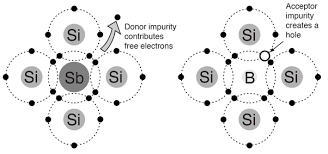
\includegraphics{download.png}
   \end{center}
    \begin{center}
      \emph{n-type and p-type doped semiconductor crystal}
  \end{center}
\par

In order to understand doping effects, we must also analyze the effects of external impurities on band diagram of the semiconductor. It turns out that on doping, the Fermi level inside the semiconductor changes, which is a consequence of the deviation of carrier concentrations from the intrinsic carrier concentration, $n_{i}$. In a n-type doped material, the $E_{F}$ gets closer to the conduction band whereas in a p-type doped material, $E_{F}$ gets closer to the valence band. As a result, from the formulae for $n_{e}$ and $n_{h}$, we can observe that $n_{e} > n_{h}$ for a n-type material and vice-versa for a p-type material as we expected physically too.\newline

  \par
   \begin{center}
  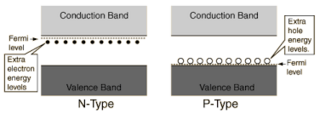
\includegraphics{doping_2_85.png}
  \end{center}
    \begin{center}
      \emph{n-type and p-type doped semiconductor crystal}
  \end{center}
\par

The exact relation between n, p, $N_{A}$, $N_{D}$(without the assumption that $N_{D} >> n_{e}$ or $N_{A} >> n_{h}$)can be established using the concept of charge neutrality and the relation $n\cdot p = n_{i}^{2}$. Thus, the equation goes as follows:
\begin{center}
    $n + N_{A}^{-} = p + N_{D}^{+}  $
\end{center}
Assuming complete ionization of donor and/or acceptor atoms, $N_{A}^{-} = N_{A}$ and $N_{D}^{+} = N_{D}$. Now, substituting $n\cdot p = n_{i}^{2}$ in the equation,

\begin{center}
    $ \frac{n_{i}^{2}}{n} + N_{D} = n + N_{A}  $
\end{center}

\begin{center}
    $ n^{2} + n(N_{A}-N_{D}) - n_{i}^{2} = 0  $
\end{center}

On solving this quadratic equation, we obtain:
\begin{center}
    $ n =  \frac{-(N_{A}-N_{D})+\sqrt{(N_{A}-N_{D})^{2}+4n_{i}^{2}}}{2}$
\end{center}
Similarly,
\begin{center}
    $ p =  \frac{-(N_{D}-N_{A})+\sqrt{(N_{D}-N_{A})^{2}+4n_{i}^{2}}}{2}$
\end{center}\par

Earlier we have seen that under certain conditions, the Fermi-Dirac integral involved in $n_{i}$ can be simplified. A relatively advanced approximation method also covers the cases when $E_{c}-E_{F} \leq 3k_{B}T$ or $E_{F}-E_{v} \leq 3k_{B}T$, also known as the Joyce-Dixon approximation. According to this,
\begin{center}
$ln(\frac{n}{N_{c}}) + \frac{1}{\sqrt{8}}\frac{n}{N_{c}} = \frac{E_{F}-E_{c}}{k_{B}T}$
\end{center}

\begin{center}
 $ln(\frac{p}{N_{v}}) + \frac{1}{\sqrt{8}}\frac{p}{N_{v}} = \frac{E_{v}-E_{F}}{k_{B}T}$   
\end{center}



\section{Drift and Diffusion processes of Carriers}

The two major processes through which an electric current flows inside the semiconductor is by drift and \href{https://en.wikipedia.org/wiki/Diffusion}{diffusion} processes. While the process of drift is fundamentally similar in both conductors and semiconductors, diffusion is something that is unique to semiconductors.

\subsection{Drift and mobility of carriers}

Electrons and holes that are undergoing random thermal motion inside the semiconductor cannot conduct electricity since their net displacement over a long interval of time is zero. Under application of an external electric field, the random thermal walk of electrons is superimposed with a net displacement due to the electric field's influence and thus, can constitute a current. \newline

  \par
   \begin{center}
   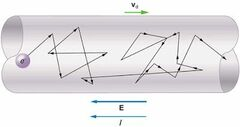
\includegraphics{drift_velocity_60.jpg}
   \end{center}
    \begin{center}
      \emph{Electron undergoing collisions with atoms in the lattice}
  \end{center}
\par

During the random thermal walk, electrons interact with the lattice in two manners-  i) through collision with vibrating atoms in the lattice, ii) through electrostatic interaction with ionized impurities. The 'collisions' here merely refer to the interaction of the electron with a potential field and not any form of physical collision taking place. Vibrating atoms interact with the electrons and holes in the lattice through particles known as \href{https://en.wikipedia.org/wiki/Phonon}{'phonons'}.\par

Using the relation between drift velocity and applied electric field, we know that:
\begin{center}
    $ v = (\frac{q\tau}{m^{*}})E $
\end{center}
where $\tau$ represents the average time between successive collision events and $m^{*}$ represents effective mass of the electron. The quantity $\frac{q\tau}{m^{*}}$ represents 'mobility' of the carrier inside the semiconductor.\par

Despite the fact that drift velocity and electric field are directly proportional to each other, at very high field values the drift velocity saturates to a maximum possible velocity, $v_{sat}$. This is because with increase in field values, the frequency of collisions with lattice increases manifolds and this acts as a limiting factor for drift velocity. Typical mobility values for semiconductors are usually in the range of $200-400          cm^{2}V^{-1}s^{-1}$. However, novel materials like \href{https://en.wikipedia.org/wiki/Graphene}{graphene} can have very high values of mobility, typically in the range of $50,000-100,000    
 cm^{2}V^{-1}s^{-1}$.\par

The two factors affecting mobility- collisions with the lattice and coulombic interaction with ionized centres behave quite differently as the temperature varies.\par
\textbf{(i) Atomic vibrations}: As temperature increases, electrons collide more frequently with atoms, hence their mobility due to atomic vibrations decreases.\par
\textbf{(ii) Ionized atoms}: As temperature increases, the thermal velocity of the electrons increases and they find it easier to overcome the Coulombic barrier of ionized dopant atoms. Hence, the mobility due to ionized impurities increases with increasing temperature.\par
The net mobility ($\mu_{tot}$), mobility due to phonon's interaction ($\mu_{phonon}$) and mobility due to ionized impurities ($\mu_{I.Imp}$) are related as:
\begin{center}
    $ \mu_{tot}^{-1} = \mu_{phonon}^{-1} + \mu_{I.Imp}^{-1}  $
\end{center}

  \par
   \begin{center}
   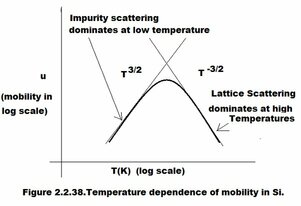
\includegraphics{mobility_temp_50.jpeg}
   \end{center}
    \begin{center}
      \emph{\hspace{2.5cm}Variation of mobility with temperature \newline}
  \end{center}
\par

\subsection{Generation-Recombination processes}

\href{https://en.wikipedia.org/wiki/Carrier_generation_and_recombination#:~:text=Carrier%20generation%20describes%20processes%20by,hole%20in%20the%20valence%20band.}{Generation} refers to the process wherein we create an electron-hole pair (EHP) from excitation of an electron from the valence band to the conduction band. \href{https://en.wikipedia.org/wiki/Carrier_generation_and_recombination#:~:text=Carrier%20generation%20describes%20processes%20by,hole%20in%20the%20valence%20band.}{Recombination} refers to the process wherein an EHP gets annihilated by an electron and the corresponding hole combining back with each other, releasing energy in the process. \par

Although the processes of generation-recombination take place intrinsically in a semiconductor, their rates can be increased by external factors such as heat, light,etc. At equilibrium and in the absence of any external stimuli, the rates of recombination and generation are exactly equal to each other, and hence, there is a constant carrier concentration w.r.t time in the semiconductor throughout. \par

\subsubsection{Direct recombination}

Semiconductors can be broadly classified under two categories- direct band-gap semiconductors and indirect band-gap semiconductors. The essential difference between the two is that in direct band-gap materials, there are no intermediate energy levels (also known as \emph{traps}) to wherein the electron may transition while being excited from the V.B. to C.B.. Direct band-gap materials are useful for light emission since nearly all the energy released during transition is in the form of photon energy, $h\nu$ (where $h\nu$ = $E_{G}$). Hence most of the materials used in LEDs such as GaAs, GaN, InGaN, etc. are direct band-gap materials. \par

When recombination occurs in direct band-gap materials, it is much faster than in the case of indirect band-gap materials since electrons do not have to undergo intermediate transitions in this case. We can say that the rate of thermal generation of carriers is proportional to the product $n_{o}p_{o}$ (or equivalently $n_{i}^{2}$) while the rate of recombination is proportional to $n(t)p(t)$ (where $n(t)$ and $p(t)$ refer to the non-equilibrium, time-dependent carrier concentrations). Also, thew proportionality constants of both these processes may be taken to be the same since they depend on the same physical factors. \par

In order to derive how non-equilibrium carrier concentrations (induced by external factors) change with time, let us consider a case where a short, high-energy pulse of light is shined on a semiconductor material. This generates let say $\Delta n$ and $\Delta p$ excess carrier concentrations in addition to the initial $n_{o}$ and $p_{o}$ carriers. The excess carriers decay as $\delta n(t)$ and $\delta p(t)$ in time. We know that since the sample was initially at equilibrium(considering only electrons as of now),
\begin{center}
    $ \frac{dn(t)}{dt} = \alpha n_{i}^2 - \alpha n(t)p(t) = 0$
\end{center}
After shining light on the sample,
\begin{center}
    $  \frac{dn(t)}{dt} = \alpha n_{i}^{2} - \alpha [n_{o}+\delta n(t)][p_{o}+\delta p(t)] $
\end{center}

\begin{center}
    $ => \frac{dn(t)}{dt} = -\alpha [(n_{o}+p_{o})\delta n(t) + \delta n^{2}(t)]  $
\end{center}
Ignoring the quadratic term,
\begin{center}
    $ \frac{dn(t)}{dt} = -\alpha (n_{o}+p_{o})\delta n(t) $
\end{center}

Now, since $n(t)$ = $n_{o} + \delta n(t)$, this implies that $ \frac{dn(t)}{dt} = \frac{d\delta n(t)}{dt}$. Using this fact, the equation obtained above can be easily solved to obtain an exponentially decaying excess carrier concentration in the sample.
\begin{center}
    $ \delta n(t) = \Delta ne^{-\alpha p_{o}t} = \Delta ne^{-t/\tau_{n}}  $
\end{center}
where $\Delta n$ refers to the initial concentration of excess carriers generated at t$=0$ and $\tau_{n} = (\alpha p_{o})^{-1}$ is known as the \emph{recombination lifetime} of the electron. These same equations hold for holes too, with minor changes in variables. \par

\subsubsection{Trap statistics and indirect recombination}

Traps in a semiconductor lattice are physical defects, dislocations etc. in the lattice that can create additional energy levels in the crystal and thus, affect carrier concentrations. These energy levels can capture/emit electrons or holes, which affects the equilibrium carrier concentration. The probability that a trap energy state, $E_{t}$ is occupied is given as:
\begin{center}
    $ f(E_{t}) = \frac{1}{1+exp(\frac{E_{t}-E_{F}}{k_{B}T})}$
\end{center}
Indirect band-gap semiconductors have a significant concentration of trap energy states, which is why the electrons being excited from the V.B. to C.B. do not get to reach the C.B. directly. Instead, some of the electrons initially transition into a trap energy state lower than the C.B. and undergo further transition to C.B. from there. This delays the transition time from the expected theoretical value and such semiconductor materials are not suitable for light emission. \newline

  \par
  \begin{center}
   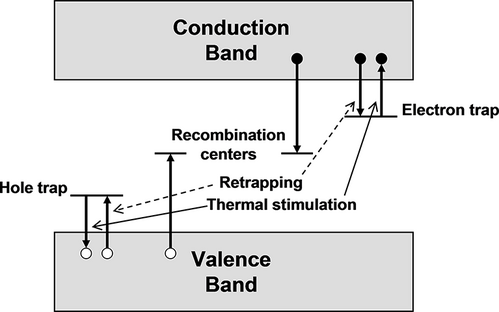
\includegraphics{fig1_1_65.png}
   \end{center}
    \begin{center}
      \emph{\hspace{1.5cm}Energy band diagram showing electron and hole traps\newline}
  \end{center}
\par

The rate of electron (or hole) capture by traps depends upon the thermal velocity of electrons ($v_{th}$), electron concentration (n), probability of finding a trap state to be empty and the capture cross-sectional area of the trap,$\sigma_{n}$ (Capture cross-sectional area refers to the region of influence of the trap which possesses a high probability of capturing an electron passing through it). Hence, the rate of electron capture, $r_{a}$ can be written as:
\begin{center}
    $ r_{a} = \sigma_{n}v_{th}nN_{t}(1-f) $
\end{center}
where $N_{t}$ is the total number of trap states and f represents the probability of a trap state being occupied.\par
Similarly, the rate of electron (or hole) emission by traps, $r_{b}$ is given by:
\begin{center}
    $ r_{b} = \lambda N_{t}f $
\end{center}
where $\lambda$ is some proportionality constant.

\subsection{Diffusion of carriers}

\href{https://en.wikipedia.org/wiki/Diffusion_current}{Diffusion} of charge carriers constitutes the diffusion current in semiconductors. It occurs due to the non-uniform, space-varying concentration of charge carriers (which might otherwise be at equilibrium). This process of diffusion is described by \href{https://en.wikipedia.org/wiki/Fick%27s_laws_of_diffusion}{Fick's law}. In order to understand the process, consider the graph below depicting a non-uniform carrier concentration which varies along the x-direction (uni-dimensional diffusion).\newline

  \par
  \begin{center}
  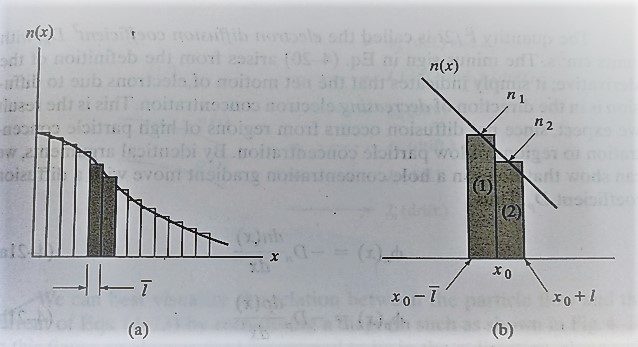
\includegraphics{Adobe_Scan_Jun_17_2022_page-0001_1_50.jpg}
  \end{center}
   \begin{center}
       \emph{\hspace{0.8cm}Graph showing variation of carrier concentration with x-coordinates\newline}
   \end{center}
\par

Consider the graph to be made up of a number of smaller rectangles, each of width $\overline{l}$, where $\overline{l}$ represents the average distance covered by the electrons between subsequent collisions. Now, consider the two small rectangles $(1)$ and $(2)$ shaded out in fig.(a). Let the electron concentrations in $(1)$ and $(2)$  be $n_{1}$ and $n_{2}$, respectively. Let $\tau$ be the relaxation time (average time between successive collisions). Consider the common boundary between the two rectangular bars. The net flux of electron through this cross section is non-zero since the carrier concentration is different on both sides. At any moment of time, about half of the electrons enclosed within the rectangular regions would be crossing the boundary from each side. Hence, the net flux through the surface can be expressed as:
\begin{center}
    $ \phi_{n}(x_{o}) = \frac{\overline{l}}{\tau}\frac{n_{1}-n_{2}}{2}  $
\end{center}
Using fundamental ideas of calculus, it can be shown that:
\begin{center}
    $  n_{1} - n_{2} = \frac{n(x) - n(x+\Delta x)}{\Delta x}\overline{l}   $
\end{center}
Therefore,
\begin{center}
    $ \phi_{n}(x_{o}) = \frac{\overline{l}^{2}}{2\tau} \frac{n(x) - n(x+\Delta x)}{\Delta x}\overline{l}   $
\end{center}
In the limit of $\Delta x -> 0$, the expression can be further simplified as:
\begin{center}
    $ \phi_{n}(x_{o}) = -\frac{\overline{l}^{2}}{2\tau}\frac{dn(x)}{dx}   $
\end{center}
The quantity $\frac{\overline{l}^{2}}{2\tau}$ is also known as the \emph{electron diffusion coefficient}, $D_{n}$. From the minus sign, we may infer that the flux of the electrons is from regions of higher concentration to regions of lower concentration. Similar equations can also be written for holes, with minor changes in variables.\par
\begin{center}
    $ \phi_{n}(x_{o}) = -D_{n}\frac{dn(x)}{dx}  $
\end{center}
\begin{center}
    $ \phi_{p}(x_{o}) = -D_{p}\frac{dp(x)}{dx} $
\end{center}

Now that we have the equations for carrier flux through the boundary, one can easily define the current density at any given point. Therefore,
\begin{center}
    $  J_{n} = (-q)(-D_{n}\frac{dn(x)}{dx}) = qD_{n}\frac{dn(x)}{dx}  $
\end{center}
\begin{center}
    $  J_{p} = (q)(-D_{p}\frac{dp(x)}{dx}) = -qD_{p}\frac{dp(x)}{dx} $
\end{center}
Therefore, the net diffusion current density is given as:
\begin{center}
    $   J_{diff} = J_{n} + J_{p} = qD_{n}\frac{dn(x)}{dx} - qD_{p}\frac{dp(x)}{dx}   $
\end{center}

\subsubsection{Einstein Relation}

\href{https://en.wikipedia.org/wiki/Einstein_relation_(kinetic_theory)}{Einstein relation} acts as a link between the drift and diffusion currents in a semiconductor at equilibrium through which no net current is flowing. As we know,
\begin{center}
    $ n(x) = N_{c} exp(\frac{E_{F}-E_{c}(x)}{k_{B}T})  $
\end{center}
\begin{center}
    $ E(x) = \frac{1}{q}(\frac{dE_{c}(x)}{dx}) $
\end{center}
where $E(x)$ represents the electric field inside the semiconductor due to the slope in the energy levels of C.B. and V.B.. Now, equating the sum of drift and diffusion currents of the individual carriers to zero, we obtain,
\begin{center}
    $  qD_{n}(x)\frac{dn(x)}{dx} + q\mu_{n} n(x)E(x) = 0  $
\end{center}
From the expression for n(x), we obtain,
\begin{center}
    $  \frac{dn(x)}{dx} = N_{c}(-\frac{1}{k_{B}T})exp(\frac{E_{F}-E_{c}(x)}{k_{B}T})\frac{dE_{c}(x)}{dx} = n(x)(-\frac{1}{k_{B}T})\frac{dE_{c}(x)}{dx}  $
\end{center}
Substituting back into the original equation,
\begin{center}
    $ D_{n}n(x)(-\frac{1}{k_{B}T})\frac{dE_{c}(x)}{dx} + \mu_{n} n(x)\frac{1}{q}\frac{dE_{c}(x)}{dx} = 0  $
\end{center}
\begin{center}
 $ D_{n} = \frac{k_{B}T}{q}\mu_{n} , D_{p} = \frac{k_{B}T}{q}\mu_{p}  $
\end{center}
This relation between diffusion coefficients and mobility suggests that diffusion and drift processes are both interrelated.

\subsubsection{Continuity equation}
The \href{https://en.wikipedia.org/wiki/Continuity_equation}{continuity equation} is one of the most fundamental equations in physics and engineering applications. While continuity equation for flow of currents inside conventional conductors is quite simple, in semiconductors it is more involved since generation and recombination processes may produce/annihilate charge carriers inside the semiconductor, so that current density may not be constant over space.\par

Consider a rectangular block of semiconductor slab and take a thin slice of it of thickness $\Delta x$, perpendicular to the current density vector. Let rate of generation of electrons inside the region be $G_{L}$ and rate of recombination be $\frac{\Delta n}{\tau}$ (derived from the fact that $\Delta n= \Delta n_{o}e^{-t/\tau}$). Hence,

\begin{center}
    $ \frac{dn}{dt} = \frac{1}{q}\diffp{J_{n}(x)}{x} + G_{L} - \frac{\Delta n}{\tau} $
\end{center}

Now, $J_{n}(x) = qD_{n}\frac{dn}{dx} + q\mu nE$. Assuming E = 0,
\begin{center}
    $ \frac{dn}{dt} = \frac{1}{q}\diffp{(qD_{n}\diffp{n}{x})}{x} + G_{L} - \frac{\Delta n}{\tau}  $
\end{center}
\begin{center}
    $ \frac{dn}{dt} = D_{n}\diffp[2]nx + G_{L} - \frac{\Delta n}{\tau}   $
\end{center}
Under steady state conditions, $\frac{dn}{dt} = \frac{dp}{dt} = 0$. Also, $n = n_{o} + \Delta n$. Combining thses two facts, the above equation can be written as: 
\begin{center}
    $ D_{n}\frac{d^{2}\Delta n}{dx^{2}} + G_{L} - \frac{\Delta n}{\tau} = 0 $
\end{center}
Further assuming that the rate of generation of carriers is set to zero (i.e. $G_{L} = 0$),
\begin{center}
    $ \frac{d^{2}\Delta n}{dx^{2}} = \frac{\Delta n}{D_{n}\tau}  $
\end{center}
which can be solved using standard methods. The quantity $D_{n}\tau$ is expressed as the square of $L_{n}$, where $L_{n} = \sqrt{D_{n}\tau}$ represents the diffusion length of the carrier inside the material.\par
\begin{center}
    $ \frac{d^{2}\Delta n}{dx^{2}} = \frac{\Delta n}{L_{n}^{2}} $
\end{center}
The general solution to this D.E. is of the form-
\begin{center}
    $ \Delta n(x) = c_{1}e^{\frac{x}{L_{n}}}+c_{2}e^{-\frac{x}{L_{n}}} $,
\end{center}
where the coefficients $c_{1}$ and $c_{2}$ will be determined as per the boundary conditions applicable to the situation. The equation can be further simplified for practical use if we take into consideration the fact that there are, generally, two possible cases- one where the diode length is much larger than the depletion length(long diode) and the other where the diode length is much shorter than the depletion length(short diode).\par

In a short diode, the exponential terms can be simplified to their linear approximations($e^{x} = 1+x$, for $x<<1$) since $x/L_{n}<<1$. So the excess carrier concentration in this case falls off linearly. In a long diode, the coefficient of the term, $e^{\frac{x}{L_{n}}}$ must be zero since it would otherwise imply that the excess carrier concentration increases indefinitely on moving away from the origin, which is not possible theoretically. Hencce, the excess carrier concentration falls off exponentially in this case.

The continuity equation can be expressed in many formats as we have seen above. Hence, it depends a lot on the situation as to what form of the equation should be used for our purpose.

\section{P-N Junctions}

\href{https://en.wikipedia.org/wiki/P%E2%80%93n_junction}{p-n junctions} are elementary constituents of many modern electronic devices such as diodes, solar cells, rectifiers, ICs, transistors, etc. The p-n junction is essentially composed of two pieces of p-type and n-type doped material joined together at an interface. The interface between the two has to be fabricated by special means and cannot be simply constructed mechanically. \newline

 \par
  \begin{center}
   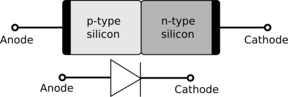
\includegraphics{1920px-PN_diode_with_electrical_symbol.svg_15.png}
   \end{center}
   \begin{center}
       \emph{\hspace{2cm}p-n junction diode and its symbol \newline}
   \end{center}
\par 

Some of the assumptions that we will be taking while dealing with p-n junctions are as follows:
(i) The material is lightly/moderately doped, (ii) Complete ionization of dopant atoms, (iii) All calculations are made at ideal operating conditions, i.e. at room temperature. \par

\subsection{p-n junction at equilibrium}

Due to concentration gradient across the junction, a diffusion current starts flowing across it. However, at the junction itself, electrons and holes capture each other and thus, recombine, resulting in the release of energy. This process of recombination depletes the region adjacent to the junction of electrons and holes, leaving behind an excess of immobile dopant atoms and therefore, it is also known as the depletion region. These immobile atoms now create an in-built potential across the junction which is opposite to the flow of the diffusion current. This in-built potential steadily grows with time until the diffusion current can no longer flow across the junction. Hence, even without any application of external potential, there exists an in-built potential, say $V_{bi}$ across the p-n junction.\par

When a p-n junction is under equilibrium, the Fermi level on both p- and n-side is \emph{invariant} with position. This is a consequence of the fact that rates of generation and recombination exactly balance each other at equilibrium and can be proved. The C.B.s and V.B.s of the two sides merge with each other in a continuous fashion, keeping band-gap energy constant throughout as shown in the figure below: \newline

 \par
  \begin{center}
   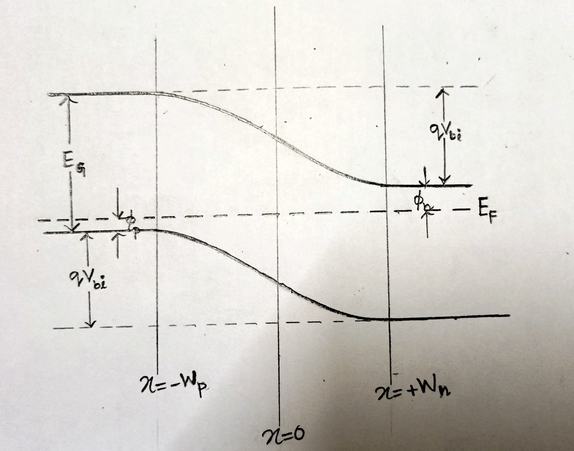
\includegraphics{hand_drawn_2_45.jpg}
     \end{center}
   \begin{center}
       \emph{\hspace{2cm}Energy band diagram of a p-n junction\newline}
   \end{center}
\par

Let the width of the depletion region be $ W = W_{n} + W_{p}$ where $W_{n}$ and $W_{p}$ represent the widths of the depletion region on n- and p-sides respectively. Let $\phi_n$ and $\phi_p$ represent the energy gap between $E_{c}$ and $E_{F}$ on n-side and $E_{v}$ and $E_{F}$ on p-side respectively. We know that,
\begin{center}
    $\phi_n = k_{B}T ln(\frac{N_{c}}{N_{D}}) $
\end{center}
\begin{center}
    $\phi_p = k_{B}T ln(\frac{N_{v}}{N_{A}})   $
\end{center}

From observation, one can reach the conclusion that:
\begin{center}
    $  qV_{bi} = E_{G} - \phi_{n} - \phi_{p} $
\end{center}

\begin{center}
    $ qV_{bi} = E_{G} - k_{B}T ln(\frac{N_{c}N_{v}}{N_{a}N_{D}}) = E_{G} - k_{B}T ln(\frac{N_{c}N_{v}}{np}) $
\end{center}

Now, 
\begin{center}
    $ n_{i}^{2} = N_{c}N_{v}exp(-\frac{E_{G}}{k_{B}T})  $
\end{center}
Substituting this in the previous equation and eliminating $E_{G}$,
\begin{center}
    $  V_{bi} = \frac{k_{B}T}{q} ln(\frac{N_{A}N_{D}}{n_{i}^{2}})    $
\end{center}
which gives us an estimate for the built-in potential in terms of dopant concentrations. We can also derive a relation between $V_{bi}$ and the width of the depletion region using \href{https://en.wikipedia.org/wiki/Poisson%27s_equation}{Poisson's equation}.\par
Since the sample must remain electrically neutral throughout the process, net charge must be zero within the depletion region. This implies that $ N_{A}W_{p} = N_{D}W_{n}$. This also means that higher the doping on a given side, lower is the depletion width on that side. Now, applying Poisson's equation to the n-side, 
\begin{center}
    $ \frac{d^{2}V}{dx^{2}} = -\frac{\rho}{\epsilon_{o}\epsilon_{r}}   $
\end{center}
This implies:
\begin{center}
    $  \frac{dE}{dx} = \frac{qN_{D}}{\epsilon_{o}\epsilon_{r}}   $
\end{center}
On integrating with the appropriate limits,
\begin{center}
    $  E = \frac{qN_{D}}{\epsilon_{o}\epsilon_{r}}(x-W_{n})  $, for $0 < x \leq   W_{n}$
\end{center}
Similarly, 
\begin{center}
    $ E = -\frac{qN_{A}}{\epsilon_{o}\epsilon_{r}}(x+W_{p})    $, for $-W_{p} \leq x < 0$
\end{center}

Now, having found the electric field in the depletion region, we are in a position to determine the built-in potential difference across the junction. 
\begin{center}
    $ V_{bi} = -(\int_{-W_{p}}^{0} E\,dx + \int_{0}^{W_{n}} E\,dx)     $
\end{center}
On solving this particular integral, we obtain,
\begin{center}
    $  V_{bi} = \frac{q}{2\epsilon_{o}\epsilon_{r}}(N_{A}W_{p}^{2} + N_{D}W_{n}^{2})   $
\end{center}
which on further simplification, yields:
\begin{center}
    $ W = \sqrt{\frac{2\epsilon_{o}\epsilon_{r}}{q}V_{bi}(N_{A}^{-1} + N_{D}^{-1})}  $
\end{center}
where W represents the width of the depletion region. 

\subsection{p-n junction under bias}

\subsubsection{Quasi-Fermi levels} 

Before we move into the analysis of p-n junctions under bias, we need to understand the concept of quasi-Fermi levels. Quasi-Fermi levels are used to calculate the carrier concentrations in a semiconductor sample when it is under a state of \href{https://en.wikipedia.org/wiki/Quasistatic_process}{quasi-equilibrium}. \par
The Fermi level in a semiconductor can estimate the carrier concentrations at thermal equilibrium. As we know, this state of thermal equilibrium is fairly dynamic in nature-though the carrier population remains constant over time, an individual carrier simply doesn't remain at rest in a particular energy band. Due to thermal generation of EHPs, some electrons are excited into the conduction band from the valence band. At the same time, an equal number of holes from C.B. recombine with  electrons from V.B., keeping carrier populations constant over time. After an electron has been excited into a higher energy level, it undergoes rapid transitions (phonon interactions) to reach the lowest energy level in C.B. Similarly, a hole in lower regions of V.B. undergoes rapid transitions to reach the top of V.B. (Since the energy bands are w.r.t electrons, hole energy goes the other way round). These intra-band transitions take about $10^{-12}$ to $10^{-13}$ seconds. In contrast, the inter-band transitions take about $10^{-8}$ to $10^{-9}$ seconds. Such a wide range of difference in the transition times is what makes possible a quasi-equilibrium state in the semiconductor. \par
The need for introduction of quasi-Fermi levels is clearly understood through a physical analogy of water tank and pump. \par

Let us say that the energy level, $E_{c}$ and $E_{v}$ can be represented by two tanks of water where the water level in each represents the electronic concentration. The thermal generation process can be thought of as a thermal pump operating between the two tanks and pumping water from the lower tank ($E_{v}$) to the upper tank ($E_{c}$) at a given rate for a particular temperature. The recombination process can be visualised as a leaky upper tank so that some of the water pumped into the upper tank leaks to the lower tank, thereby decreasing the water level of the upper tank. At T = 0K, the thermal pump doesn't operate, so there's no change in water level (electrons) in either of the tanks (the upper tank is empty as of now). At a finite temperature, the thermal pump starts operating and pumping water into the upper tank. Some of the water leaks out into the lower tank due to the holes in the upper tank and thus, they help establish an equilibrium water level in both the tanks. \par

Now, suppose that due to external factors, there is an additional pump operating between the two tanks. Now, at the same temperature, the equilibrium water level would be different in both the tanks. The water level in lower tank falls while that in the upper tank rises. This is analogous to electrons being pumped into the C.B. by external factors, which is the same situation as in a p-n junction under bias. Thus, it can be inferred that the equilibrium Fermi level can no longer account for this new population since the temperature remains unchanged throughout the process. This is where the quasi-Fermi levels are taken into consideration.\par

Instead of a single Fermi level, we now define two different quasi-Fermi levels such that, 

\begin{center}
    $ n = N_{c}exp(\frac{E_{Fn}-E{c}}{k_{B}T}) $
\end{center}
\begin{center}
    $ p = N_{v}exp(\frac{E_{v}-E_{Fp}}{k_{B}T}) $
\end{center}
Consequently, \par
\begin{center}
    $np$ = $n_{i}^{2} exp(\frac{E_{Fn}-E_{Fp}}{k_{B}T})$
\end{center}

Hence, the value of $E_{Fn}-E_{Fp}$ serves as a measure to know how much deviation is there from the equilibrium position in the semiconductor crystal. At thermal equilibrium, the two quasi-Fermi levels merge together to form a single Fermi level. \par

\subsubsection{Forward bias}

Let us first consider the case of a p-n junction diode under forward bias. In a forward biased p-n junction diode, the majority carriers from one side are pumped to the other side due to the applied voltage. For example, electrons from n-side are pumped to the p-side, where they now become the minority carriers. Now, these minority carriers on each side recombine with majority carriers and start to decay, creating a concentration gradient in the respective regions they occupy. This concentration gradient starts a diffusion current, which can be attributed to minority carriers. In order to estimate this diffusion current, first we need to evaluate the concentration profile. And in order to do so, we need to use the concept of quasi-Fermi levels and how these quasi-levels behave under the application of an external bias. \par

Under forward bias, the quasi-Fermi levels inside the diode are separated by a gap of $qV_{a}$, where $V_{a}$ is the applied bias voltage. Away from the junction, this energy difference gradually reduces and eventually merges to a single quasi-Fermi level on both sides, i.e. at large enough distance from the junction, the carrier concentrations are restored to their equilibrium concentrations. This is depicted in the energy band diagram shown below: \newline

\par
\begin{center}
    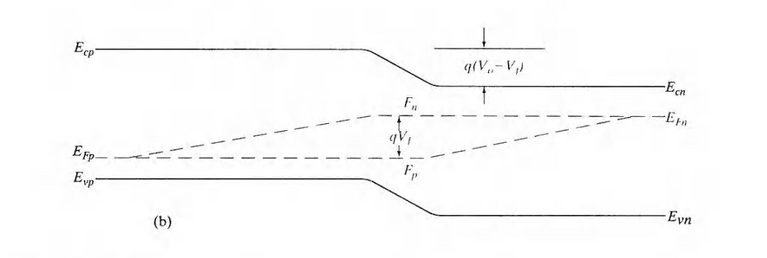
\includegraphics{diode_energy_bands_1.png}
\end{center}
\begin{center}
    \emph{\hspace{1 cm}Quasi-Fermi levels in a p-n junction diode under forward bias\newline}
\end{center}
\par

Let the dopant concentration on p-side be $N_{A}$ and the equilibrium minority carrier concentration be given by $p_{n0}$ , where $p_{n0} = n_{i}^{2}/N_{A}$ . Let $p_{n}(x)$ represent the minority carrier distribution function. Then, $p_{n}(W_{n})$ is given by- \par

\begin{center}
    $ p_{n}(W_{n}) = N_{v}exp(\frac{E_{vn}-F_{p}}{k_{B}T})  $
\end{center}

\begin{center}
    $ p_{n}(W_{n}) = N_{v}exp(\frac{E_{vn}-E_{F}}{k_{B}T})exp(\frac{qV_{a}}{k_{B}T})  $
\end{center}

Therefore, 

\begin{center}
    $  p_{n}(W_{n}) = p_{n0}exp(\frac{qV_{a}}{k_{B}T})  $
\end{center}

Hence, excess minority carrier concentration at left-hand boundary of the p-side is given by- 

\begin{center}
    $ \Delta p_{n} = p_{n0}(exp(\frac{qV_{a}}{k_{B}T})-1)  $
\end{center}

We now have two boundary conditions for the excess minority carrier concentration on n-side - at large distance from the junction, $\Delta p_{n} = 0 $ and at the junction boundary, $\Delta p_{n} = p_{n0}(exp(\frac{qV_{a}}{k_{B}T})-1) $. From continuity equation(for a long diode), we can obtain the excess minority carrier concentration profile as follows- 

\begin{center}
  $ \Delta p_{n}(x) = \frac{n_{i}^{2}}{N_{D}}(exp(\frac{qV_{a}}{k_{B}T}-1))exp(-\frac{x-W_{n}}{L_{p}})  $
\end{center}

Similarly, for the p-side, 

\begin{center}
   $ \Delta n_{p}(x) = \frac{n_{i}^{2}}{N_{A}}(exp(\frac{qV_{a}}{k_{B}T}-1))exp(\frac{x+W_{p}}{L_{n}})  $
\end{center}

The diffusion currents can now be determined directly as:

\begin{center}
    $  J_{n}(x) = qD_{n}\frac{d\Delta n(x)}{dx} = -q\frac{D_{n}}{L_{n}}(exp(\frac{qV_{a}}{k_{B}T}-1))exp(\frac{x+W_{p}}{L_{n}})$
\end{center}

\begin{center}
    $ J_{p}(x) = -qD_{p}\frac{d\Delta p(x)}{dx} = -q\frac{D_{p}}{L_{p}}(exp(\frac{qV_{a}}{k_{B}T}-1))exp(-\frac{x-W_{n}}{L_{p}}) $
\end{center}

However, an important point has been overlooked during the calculations- the net current is not constant with position, since we have not taken drift current into consideration. Ideally, due to high resistance of the depletion region(since its carrier concentration is very low), it is assumed that all of the forward bias voltage drops across it. However, due to finite, but small, resistance of the quasi-neutral regions, there is a small electric field in this region. Along with high majority carrier concentration, this small electric field can create a drift current equivalent in magnitude to the diffusion currents of minority carriers. Therefore, the current density profile is as shown below: 

\par
\begin{center}
    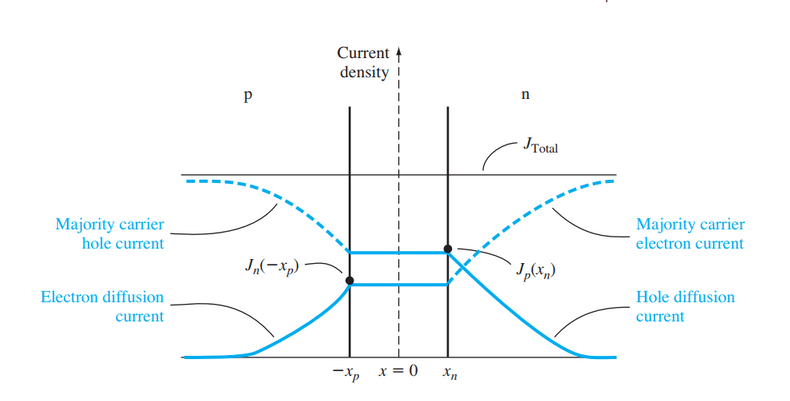
\includegraphics{pn_junction_diode_current_profile (1).png}
\end{center}
\begin{center}
    \emph{\hspace{2.5 cm}Current density profile\newline}
\end{center}
\par

At the junction boundary($x = W_{n}^{-}$ and $x = -W_{p}^{+}$), the electric field is practically zero as well as the majority carrier concentration is very low. Hence, the drift current magnitude is zero at the junction boundaries. The net current, therefore, is given by the sum of the magnitudes of the two diffusion currents at the respective junction boundaries. 

\begin{center}
    $ J_{net} = q\frac{D_{p}}{L_{p}}p_{n0}(exp(\frac{qV_{a}}{k_{B}T})-1) + q\frac{D_{n}}{L_{n}}n_{p0}(exp(\frac{qV_{a}}{k_{B}T})-1)  $
\end{center}

\begin{center}
    $ J_{net} = J_{0}(exp(\frac{qV_{a}}{k_{B}T})-1) $,
\end{center}
where $J_{0} = q\frac{D_{p}}{L_{p}}p_{n0} + q\frac{D_{n}}{L_{n}}n_{p0}$ and is known as the 'reverse saturation current'. At room temperature of 300K, $k_{B}T$ is approximately only 26 meV while $qV_{a}$ is typically much larger than this. So effectively, the current equation becomes an exponential relation between the current and applied forward voltage bias. 

\subsubsection{Reverse bias}

Mathematically, the situation in reverse bias is not quite different from forward bias- in the current equation, we can replace $V_{a}$ by $-V_{a}$ in order to evaluate the reverse bias current. Physically, what happens under reverse bias is that the minority carrier injection drastically falls due to the large potential difference existing between the two sides. Minority carriers on p-side are swept away by the large electric field to the n-side and vice-versa. This large decrease in minority carrier profile results in exponentially lower diffusion currents, and consequently, very low net current. Hence, a p-n junction practically blocks any current under reverse bias. Due to this unique property, a p-n junction is used as a 'rectifier' in circuits. \par

Due to the high electric field inside the depletion region under reverse bias situation, several interesting phenomena occur on application of high reverse voltages, notable among them being the \href{https://en.wikipedia.org/wiki/Zener_effect}{Zener breakdown} and the \href{https://en.wikipedia.org/wiki/Avalanche_breakdown#:~:text=Avalanche%20breakdown%20(or%20avalanche%20effect,a%20type%20of%20electron%20avalanche.}{avalanche breakdown}. Due to these breakdown phenomena, after a certain voltage limit(known as the breakdown voltage), the current in the diode increases tremendously even on a minuscule change in the voltage, as illustrated by the I-V characteristics. \par

Zener breakdown occurs when the high electric field inside the depletion zone enables \href{https://en.wikipedia.org/wiki/Quantum_tunnelling}{quantum tunnelling} of electrons across the depletion region, which leads to a large increase in charge carriers. Avalanche breakdown, as the name suggests, proceeds like a chain reaction. A high energy carrier can collide with an atom in the depletion zone and thus, generate an extra carrier which contributes to the current flow. This newly generated carrier can further collide with atoms, releasing more carriers. Thus, the process becomes a chain reaction(like an avalanche), which leads to a large increase in current. 

\section{Metal-Semiconductor Junctions}

\href{https://eng.libretexts.org/Bookshelves/Materials_Science/Supplemental_Modules_(Materials_Science)/Semiconductors/Metal-Semiconductors_Contacts}{Metal contacts} are a quintessential part of semiconductor devices-most of the final packaged products in the industry involve numerous metal-semiconductor junctions. Apart from this, many measurement devices, cables, etc. involve metal contacts. So, it is important to understand the characteristics of metal-semiconductor junctions in order to understand real-life semiconductor devices. \par

The two types of metal-semiconductor junctions are the '\href{https://en.wikipedia.org/wiki/Schottky_barrier}{Schottky contacts}' and the '\href{https://en.wikipedia.org/wiki/Ohmic_contact}{Ohmic contacts}'. As the name suggests, ohmic contacts obey Ohm's law while the Schottky contact's I-V characteristics resemble that of a p-n junction. That whether a given metal contact behaves as a Schottky contact or an ohmic one largely depends on the work function of the metal for a given semiconductor sample.  

\subsection{Schottky contacts}

Let us assume that the semiconductor sample under consideration is n-type doped and its Fermi level is above the Fermi level of the metal. When the metal and semiconductor sample are brought into mutual contact, electrons start to flow from the n-type material into the metal in a bid to equalize the two distinct Fermi levels at equilibrium. At equilibrium, the gap between $E_{c}$ and $E_{F}$ as well as that between $E_{v}$ and $E_{F}$ is non-uniform in the depletion region but tapers down to the initial value inside the bulk of the semiconductor. \newline

\par
\begin{center}
    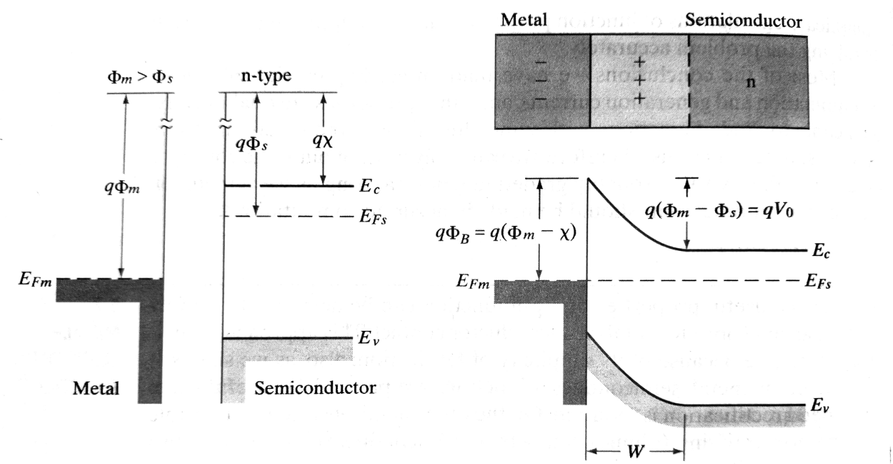
\includegraphics{Schottky_diode_n-type.png}
\end{center}
\begin{center}
    \emph{\hspace{2 cm}Schottky contact energy band diagram\newline}
\end{center}
\par

Let the Schottky contact be characterised by built-in potential $V_{bi}$, depletion width $W_{d}$, and Schottky barrier $\Phi_{B}$. Let the work functions of the metal and semiconductor be $\phi_{m}$ and $\phi_{s}$, respectively. Observe that,
\begin{center}
    $qV_{bi} = \phi_{m} - \phi_{s}$
\end{center}
Proceeding in a similar manner as in the case of p-n junctions, we can show that inside the semiconductor, Poisson's equation follows as: \par
\begin{center}
    $ \frac{d^{2}V(x)}{dx^{2}} = -\frac{qN_{D}}{\epsilon_{o}\epsilon_{s}} $
\end{center}
Which on further simplification along with the boundary condition $E(W_{d}^{+}) = 0$ yields,
\begin{center}
    $ \frac{dE(x)}{dx} = \frac{qN_{D}}{\epsilon_{o}\epsilon_{s}} $
\end{center}
\begin{center}
    $ E(x) = \frac{qN_{D}}{\epsilon_{o}\epsilon_{s}}(x-W_{d}) $
\end{center}
This yields the built-in potential as: 
\begin{center}
    $ V_{bi} = \frac{qN_{D}W_{d}^{2}}{2\epsilon_{o}\epsilon_{s}} $
\end{center}
This expression for the built-in potential is in many ways functionally similar to the one derived for the p-n junction diode. The difference between conduction band and Fermi band inside the bulk of the semiconductor is given by- 
\begin{center}
    $ E_{c}-E_{F} = \frac{k_{B}T}{q}ln(\frac{N_{c}}{N_{D}})$
\end{center}
The Schottky barrier, $\phi_{B}$, preventing the injection of electrons from metal to the semiconductor is given by-
\begin{center}
    $ \phi_{B} = qV_{bi} + (E_{c}-E_{F}) $
\end{center}
\begin{center}
    $ \phi_{B} = \frac{q^{2}N_{D}W_{d}^{2}}{2\epsilon_{s}} + \frac{k_{B}T}{q}ln(\frac{N_{c}}{N_{D}}) $
\end{center}
The Schottky contact's current equation is of the same functional form as the p-n junction diode. Therefore the Schottky contact acts as a rectifying contact like the p-n diode. In fact, in high-frequency applications the Schottky contact is preferred over the p-n junction diode. \newline

\par
\begin{center}
    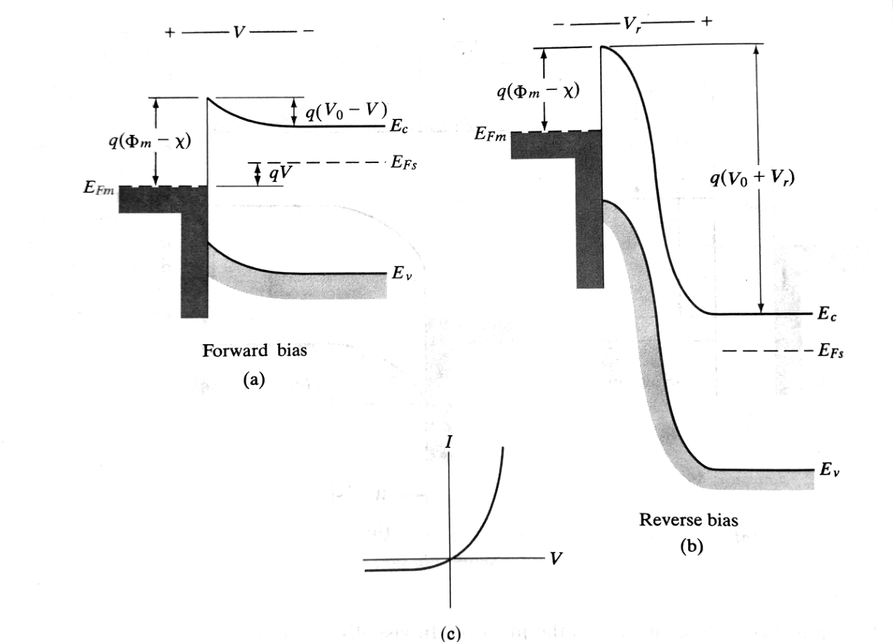
\includegraphics{Shottky_diode_bias.png}
\end{center}
\begin{center}
    \emph{\hspace{2 cm}Schottky contacts under bias\newline}
\end{center}
\par

The forward current equation in a Schottky contact is given by-
\begin{center}
    $ J = BT^{2}exp(-\frac{q\phi_{B}}{k_{B}T})exp(\frac{qV}{\eta k_{B}T})$
\end{center}
where the constant $B$ depends upon junction parameters and $1< \eta <2$. This equation is functionally similar to the current due to \href{https://en.wikipedia.org/wiki/Thermionic_emission}{thermionic emission}. 
\subsection{Ohmic contacts}

When the Fermi level of the n-type material is below the metal Fermi level, it results in an inflow of electrons from the metal to the semiconductor, resulting in an accumulation of electrons near the junction. This can also be understood in terms of energy bands as shown through the figure below: \newline

\par
\begin{center}
    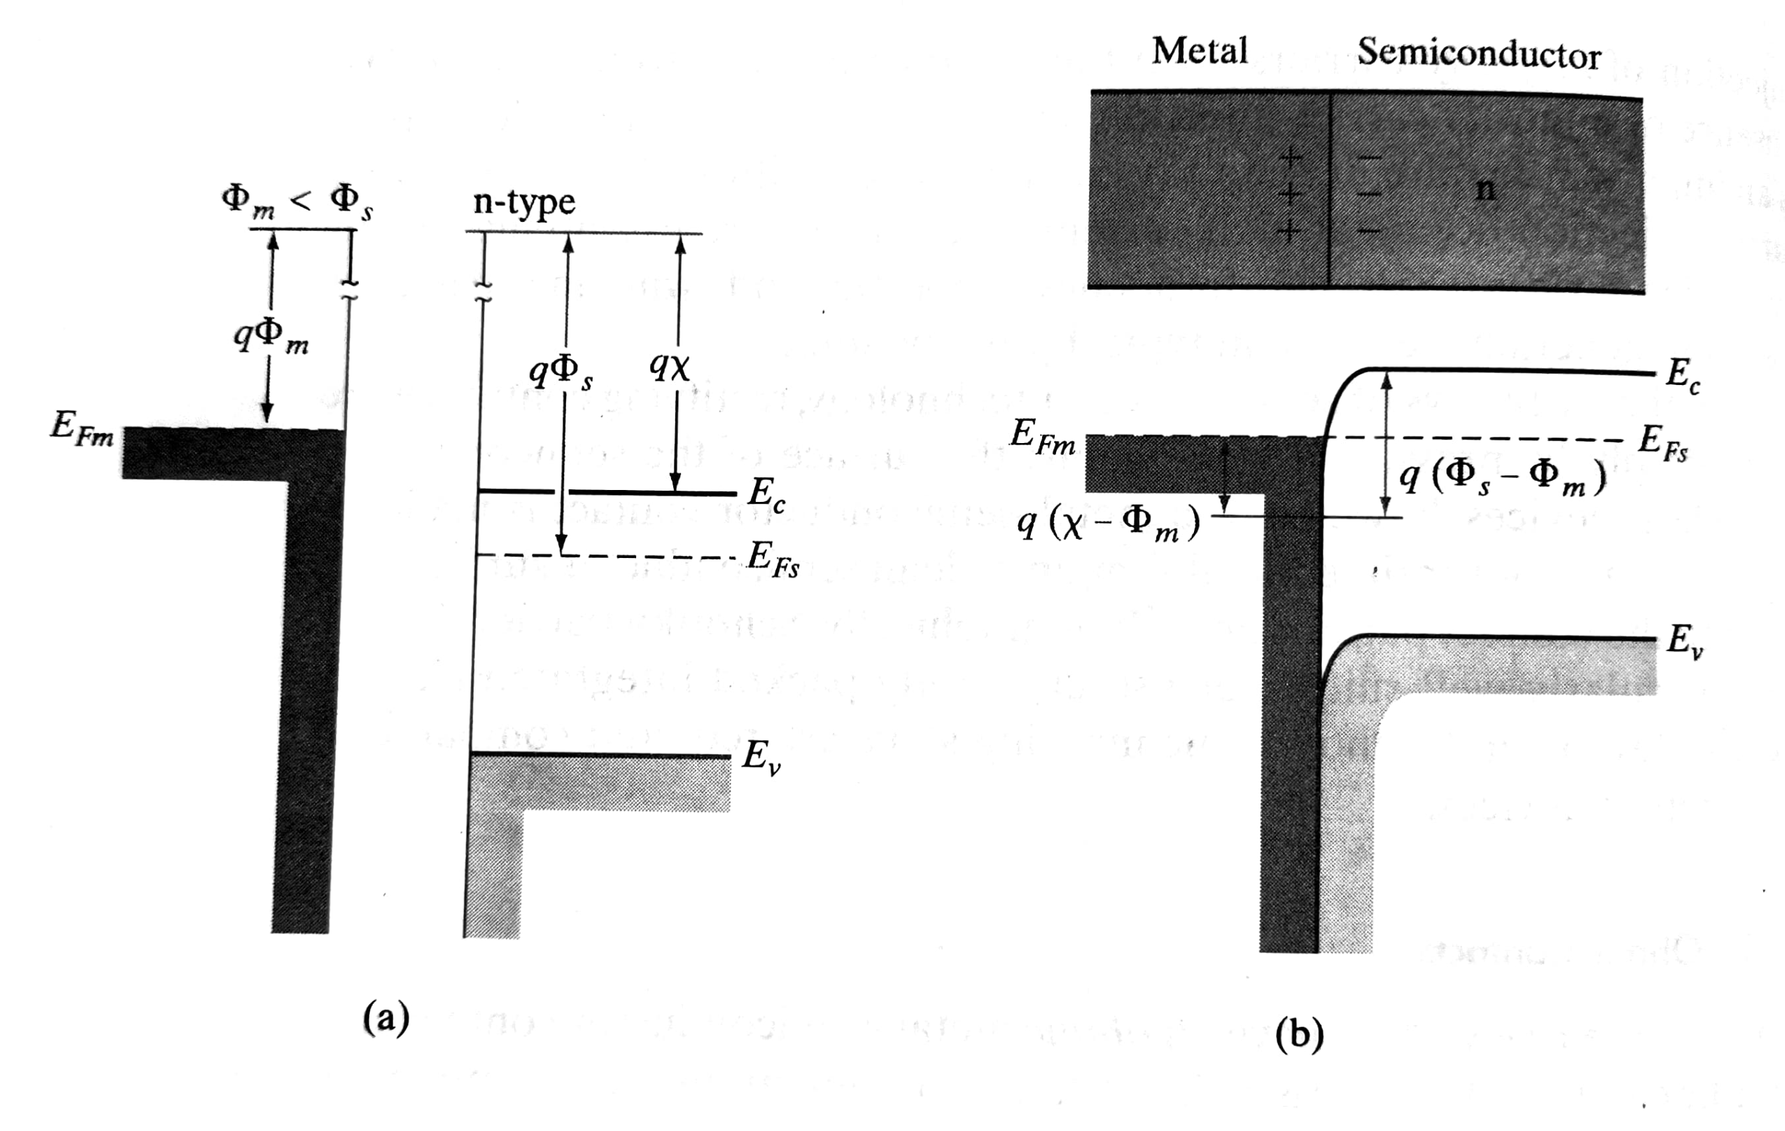
\includegraphics{Ohmic_Contact.png}
\end{center}
\begin{center}
    \emph{\hspace{2 cm}Ohmic contact\newline}
\end{center}
\par

The junction behaves as an 'Ohmic' contact because of the characteristic metal-like property associated with it - the Fermi level lying above the conduction band near the junction. \par

The cases considered till now were those of n-type semiconductors. For p-type materials, the cases are reversed - when semiconductor Fermi level lies below the metal Fermi level, it forms a Schottky contact and when it's above the metal Fermi level, it forms an Ohmic contact. These facts can be easily verified by drawing the relevant energy band diagrams. \par


\section{Metal-Oxide-Semiconductor Field-Effect Transistors(MOSFETs)}

\subsection{MOS Capacitor}

\href{https://en.wikipedia.org/wiki/MOSFET#:~:text=The%20metal%E2%80%93oxide%E2%80%93semiconductor%20field,the%20conductivity%20of%20the%20device.}{MOSFETs} and related transistors are by far the most extensively used semiconductor devices in the modern age, because of their uses in logic and memory devices. Microprocessors and memory chips include billions of MOSFETs and the number of MOSFETs included in these electronic devices is expected to double every two years, as per the well-known \href{https://en.wikipedia.org/wiki/Moore%27s_law}{Moore's Law}. \newline

\par
\begin{center}
    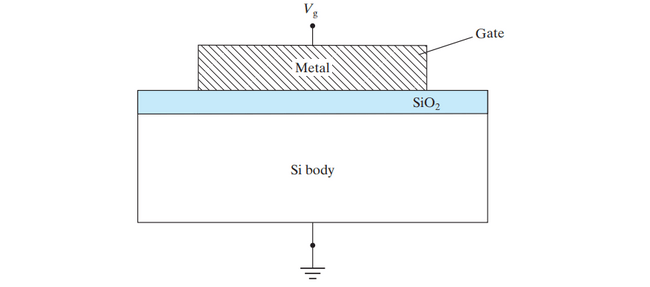
\includegraphics{MOS_capacitor_2.png}
\end{center}
\begin{center}
    \emph{\hspace{2.75 cm}MOS Capacitor\newline}
\end{center}
\par

The MOS capacitor essentially consists of a metal gate in contact with an insulator/oxide medium, which further is in contact with a p- or n-type substrate as shown in the above figure. The insulator ensures that no current flows between the metal and semiconductor. \par

There are some basic assumptions that we shall put into use while analyzing MOS capacitors (later on, we will address them). One assumption is that there is no energy difference between the metal and semiconductor Fermi levels even before joining them, i.e. flat band condition exists. The other assumption is that there are no free charges present in the bulk of insulator or the semiconductor. Under such assumptions, the energy band diagrams of the MOS capacitor are as follows: \newline

\par
\begin{center}
    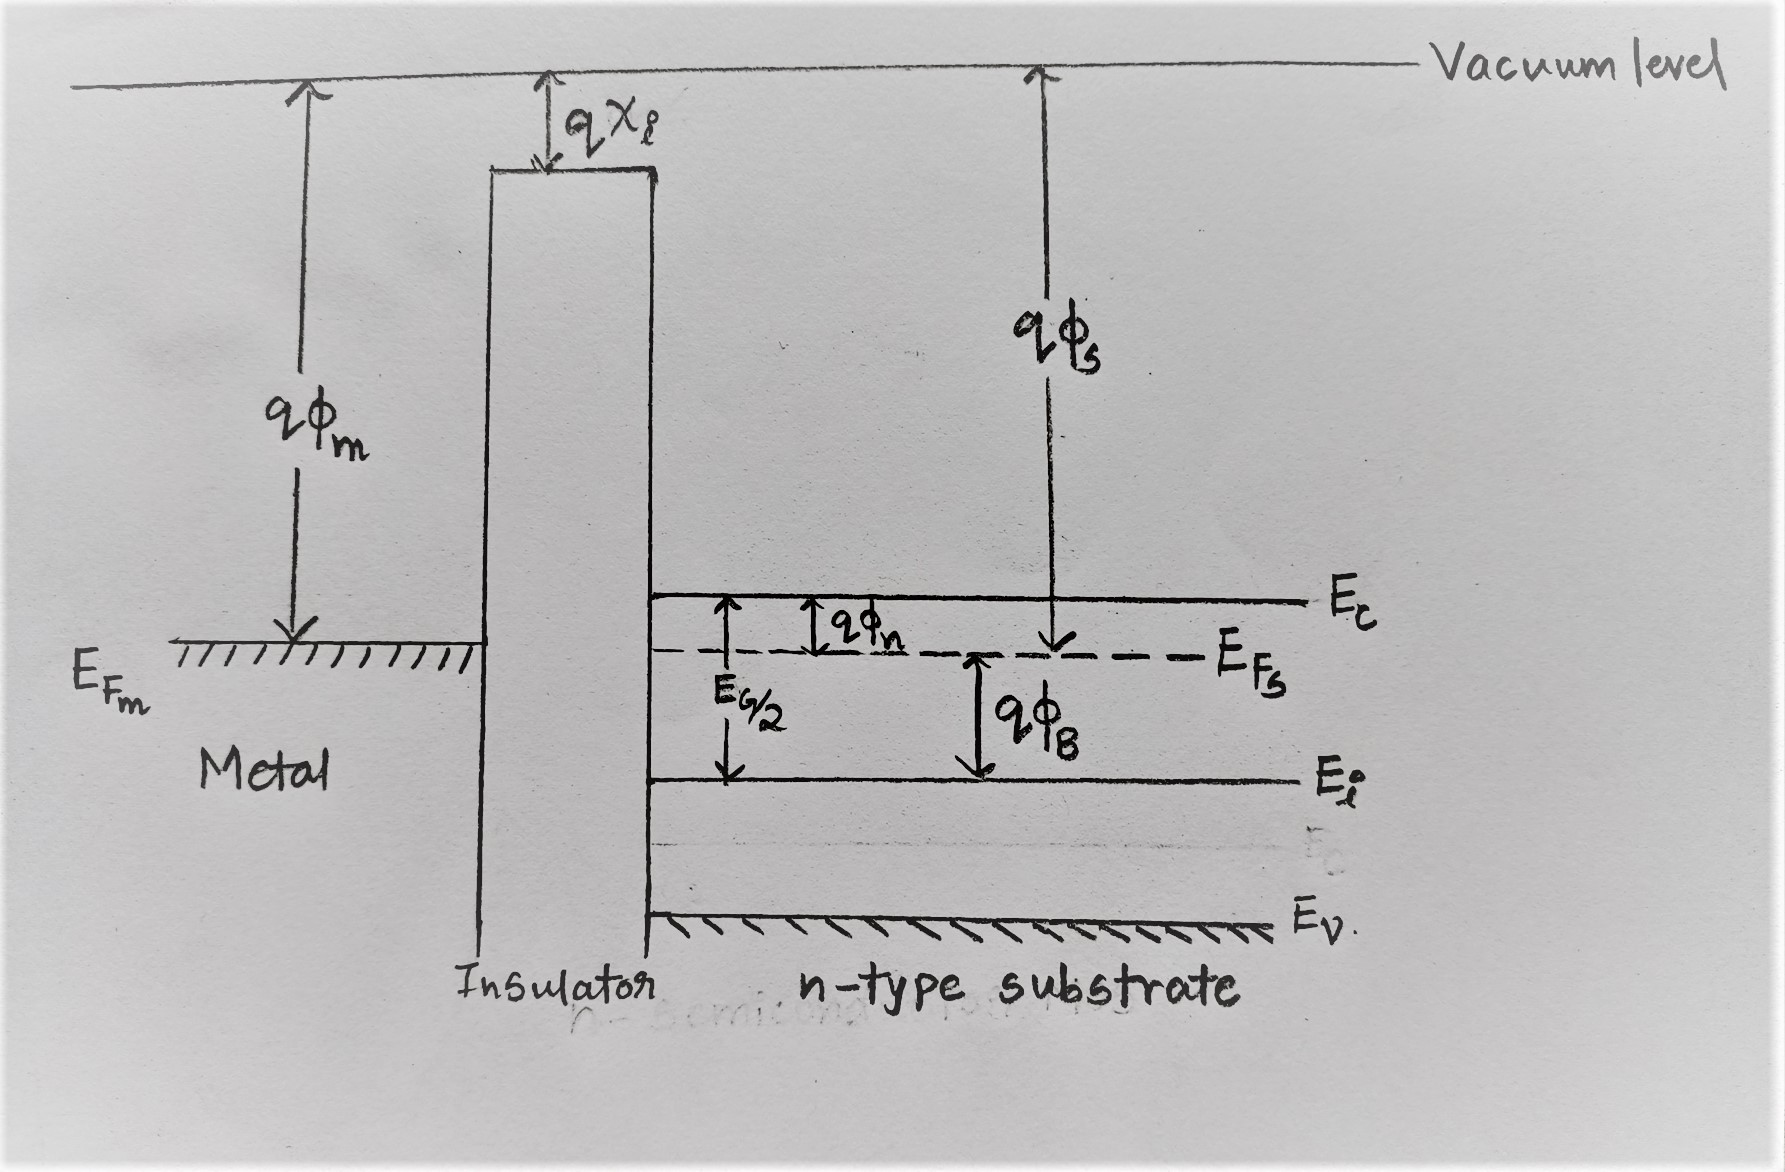
\includegraphics{MOS_energy_band_1.jpg}
\end{center}
\begin{center}
    \emph{\hspace{1.75 cm}Energy band diagram of a n-type MOS capacitor\newline}
\end{center}
\par

\par
\begin{center}
    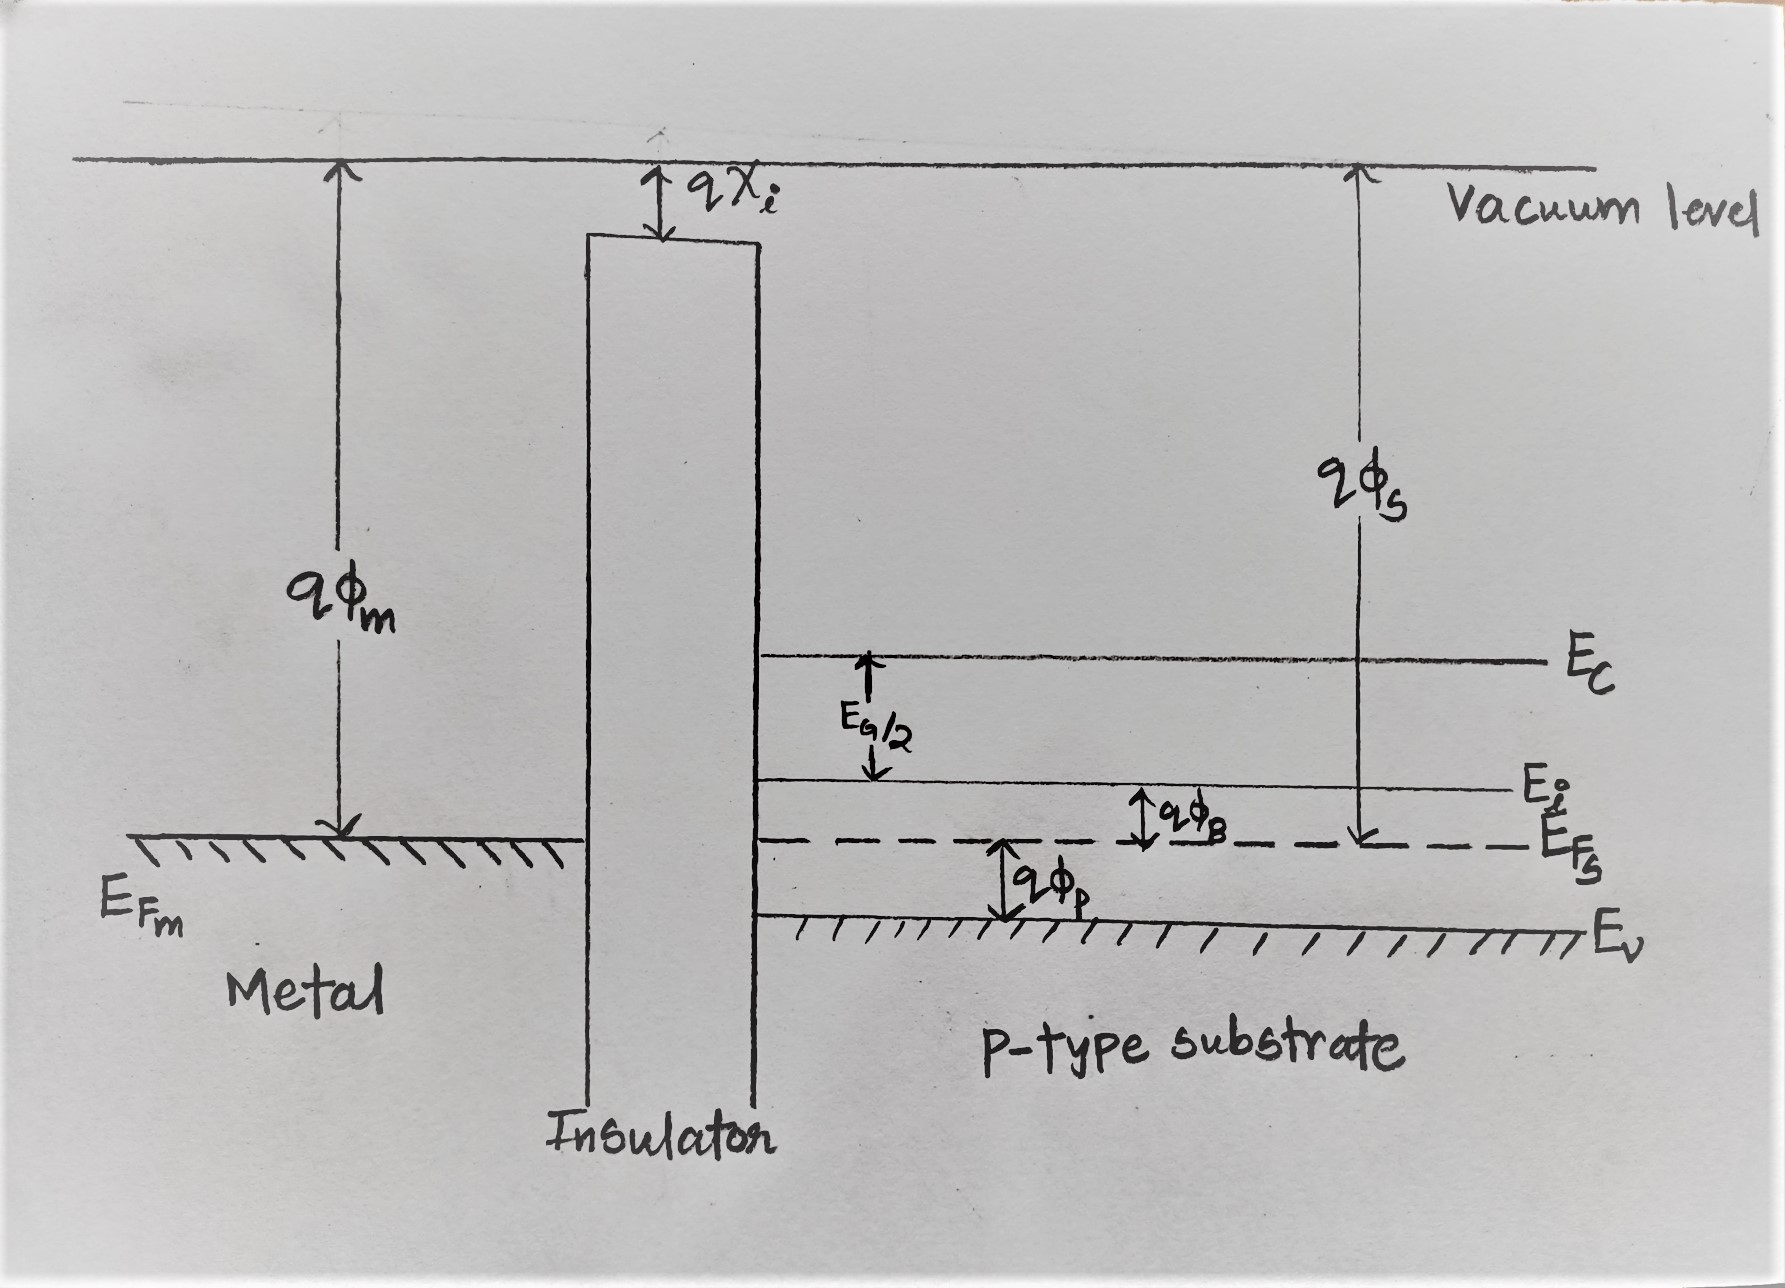
\includegraphics{MOS_energy_band_2.jpg}
\end{center}
\begin{center}
    \emph{\hspace{1.75 cm}Energy band diagram of a p-type MOS capacitor\newline}
\end{center}
\par

When a gate voltage, $V_{GS}$ is applied, there are three possibilities that may arise- accumulation, depletion or inversion. All these modes have their unique properties and associated capacitances, which have to be analyzed separately. Let us consider a p-type substrate for the associated analysis. All the results derived as such will also hold for a n-type substrate. \par

\subsubsection{Accumulation mode}

On applying a negative gate voltage, holes are drawn from the substrate to the insulator-substrate junction and consequently, a negative charge density is also induced on the metal. This process results inn band-bending of the energy levels near the junction as shown: \newline

\par
\begin{center}
    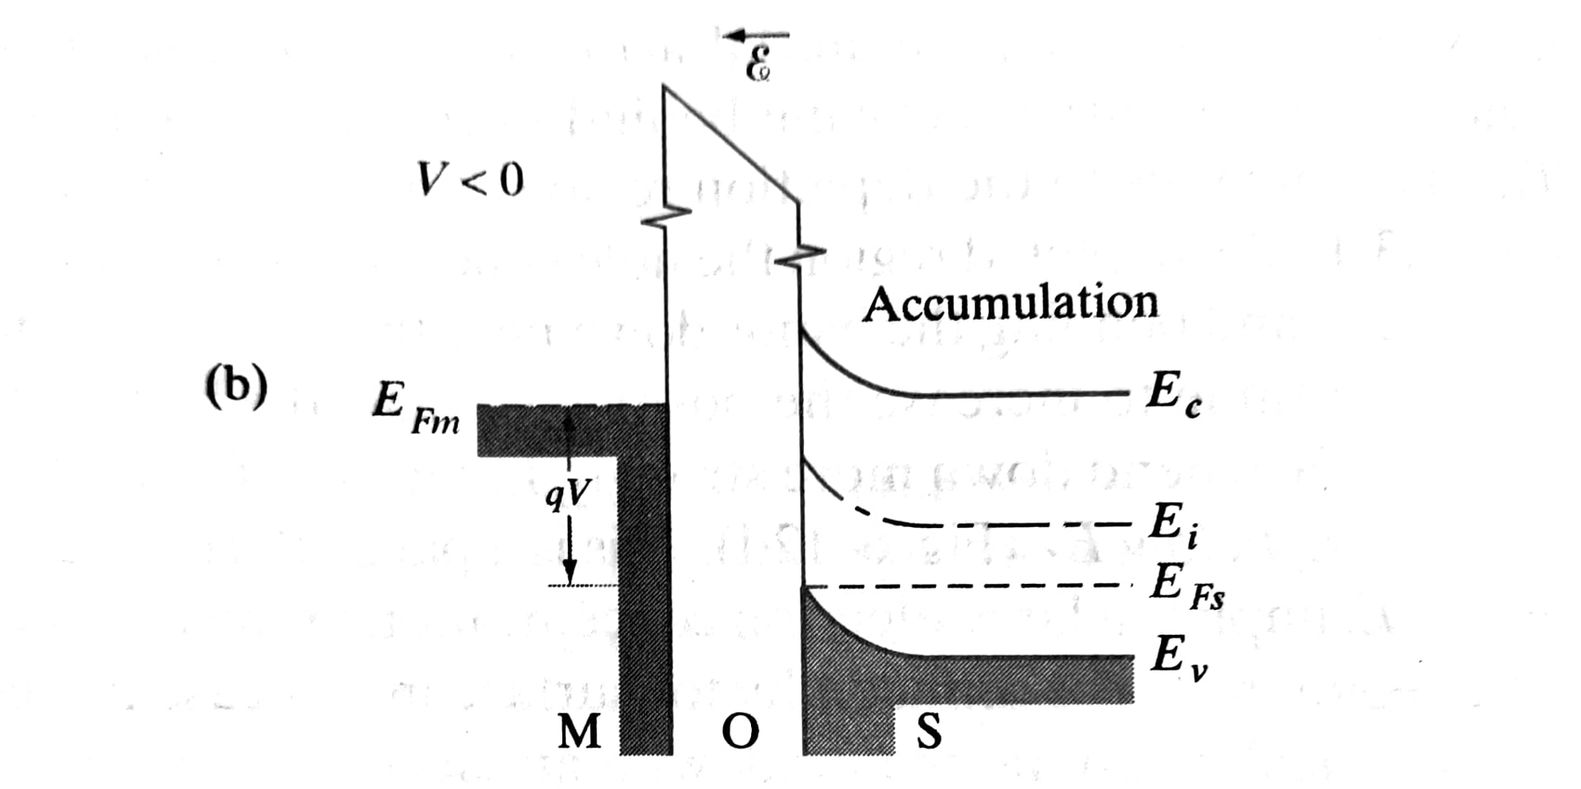
\includegraphics{Accumulation_mode_1 (5).jpg}
\end{center}
\begin{center}
    \emph{\hspace{2 cm}Energy band diagram at accumulation mode\newline}
\end{center}
\par

Since holes (majority carriers) are \emph{accumulated} near the junction, this is known as the 'accumulation' mode of operation. The gate voltage is given by-
\begin{center}
    $V_{GS} = \phi_{s} + V_{ox}$
\end{center}
Generally, $\phi_{s}$ is negligible for moderate gate voltages as compared to $V_{ox}$, so we can simplify the expression further-
\begin{center}
    $ V_{GS} \approx V_{ox} $
\end{center}
In MOS capacitor theory, unlike the electrostatic theory, we always use the substrate charge inside the semiconductor while calculating capacitances. Therefore, $V_{ox}$ is given by-
\begin{center}
    $V_{ox} = -Q_{sub}/C_{ox}$
\end{center}
this implies, 
\begin{center}
    $Q_{sub}$ = $Q_{acc}$ = $-C_{ox}V_{GS}$
\end{center}

\subsubsection{Depletion mode}

When a positive gate voltage is applied across the capacitor, the energy bands reverse their bending. The carrier population is now in quite a precarious situation- neither the hole nor the electron concentration is considerable enough to contribute to any potential difference. The holes that have been pushed away from the insulator-substrate junction leave behind a depletion region, consisting of immobile acceptor atoms, similar to the depletion region of a p-n junction diode. Hence, this mode of operation is known as the 'depletion mode'. \newline 

\par
\begin{center}
    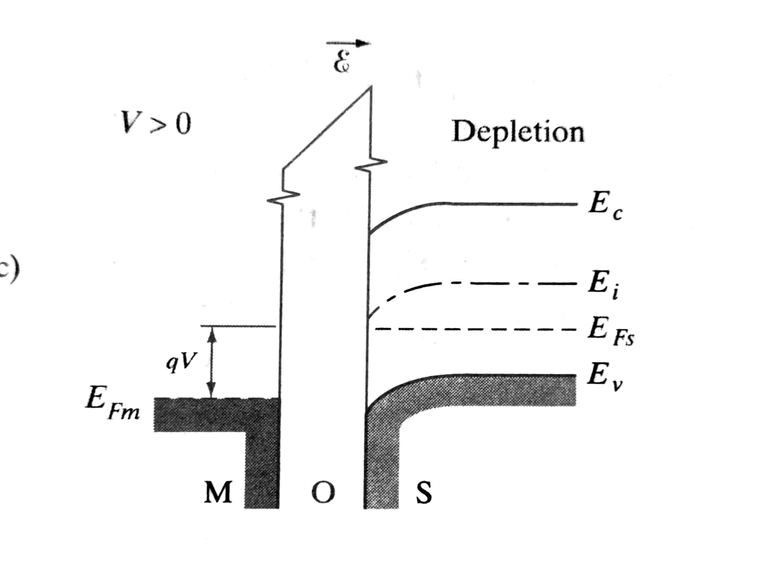
\includegraphics{Depletion _mode.png}
\end{center}
\begin{center}
    \emph{\hspace{2 cm}Energy band diagram at depletion mode\newline}
\end{center}
\par

$Q_{sub}$ is now effectively equal to $Q_{dep}$, i.e. the charge enclosed within the depletion region formed. $Q_{dep}$ is given by-
\begin{center}
    $Q_{dep} = -qN_{A}W_{d}$,
\end{center}
where $W_{d}$ is the depletion width. Now, $V_{ox}$ is given by-
\begin{center}
    $ V_{ox} = -\frac{Q_{sub}}{C_{ox}} = \frac{qN_{A}W_{d}}{C_{ox}}$
\end{center}
The relation between $\phi_{s}$ and $W_{d}$ is the same as in the case of the p-n junction diode(since the relation is a purely electrostatic one, it holds whenever there's no current density present). Therefore,
\begin{center}
    $\phi_{s} = \frac{qN_{A}W_{d}^{2}}{2\epsilon_{s}}$
\end{center}
The final expression for $V_{GS}$ is-
\begin{center}
    $V_{GS} = \frac{qN_{A}W_{d}^{2}}{2\epsilon_{s}} + \frac{qN_{A}W_{d}}{C_{ox}}$
\end{center}

One of the most important stages of the depletion mode of operation is the \emph{threshold condition}. The threshold condition represents a transition stage between the depletion and inversion modes of operation. Under this condition, the intrinsic energy level is as much below the Fermi level as it is above it. let $q\phi_{B}$ represent the gap between intrinsic and Fermi energy levels in the bulk of the semiconductor. Then, $\phi_{B}$ is given by-
\begin{center}
    $\phi_{B} = \frac{k_{B}T}{q}ln(\frac{N_{A}}{n_{i}})$
\end{center}
$\phi_{s}$ at threshold is thus given by 2$\phi_{B}$. The gate voltage is given by,
\begin{center}
    $V_{GS} = 2\phi_{B} + \frac{\sqrt{2qN_{A}\epsilon_{s}}}{C_{ox}}\sqrt{2\phi_{B}}$
\end{center}
This particular value of gate voltage is a fundamental quantity for a MOS capacitor (and for that matter, a MOSFET too) and is known as the threshold voltage, $V_{T}$. 

\subsubsection{Inversion mode}

The inversion mode of operation is when $V_{GS} > V_{T}$. Beyond this point, further increase in gate voltage leads to significant accumulation of electrons at the insulator-substrate junction. Thus, the substrate nearabout the junction is effectively 'inverted' from a p-type material to a n-type material. It is important to realize that this sheet of electrons shield off much of the electric field and therefore, any further increase in gate voltage does not affect the depletion region a lot. Rather, the excess of gate voltage from the 
threshold voltage only increases the inversion charge density. \newline

\par
\begin{center}
    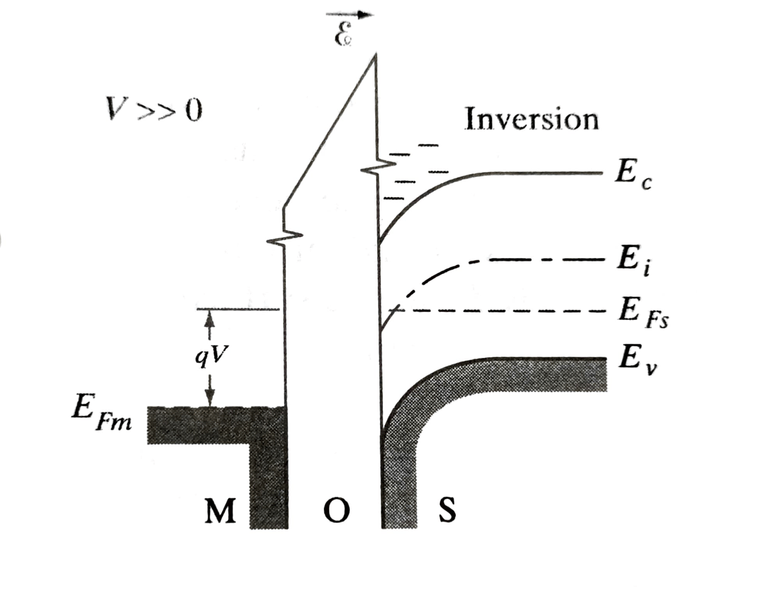
\includegraphics{Inversion_mode.png}
\end{center}
\begin{center}
    \emph{\hspace{2 cm}Energy band diagram at inversion mode\newline}
\end{center}
\par

The expression for $V_{GS}$ is now given by-
\begin{center}
    $ V_{GS} = 2\phi_{B} - \frac{Q_{dep}}{C_{ox}} - \frac{Q_{IN}}{C_{ox}}$
\end{center}
\begin{center}
    $ V_{GS} = V_{T} - \frac{Q_{IN}}{C_{ox}}$
\end{center}
That is, 
\begin{center}
    $ Q_{IN} = -C_{ox}(V_{GS}-V_{T}) $
\end{center}
In theory, it is good enough to assume that the electrons in the inversion region are readily supplied by the p-type substrate. Practically, however, due to low minority carrier concentration, it can be upto several minutes before the electrons are generated thermally to be supplied. The MOSFET overcomes this problem by having $n^{+}$-type material attached to the p-type substrate to provide the electrons readily. \par

Although we have ignored the presence of inversion charges in the neighbourhood of threshold voltage, it is not entirely correct to do so. It is quite true that the effects of the inversion charge density are significant only after the threshold voltage. However, it is also true that the inversion charge density should also be present at voltages below threshold voltage (albeit of very low magnitude). This free charge is responsible for \emph{subthreshold conduction} in the MOSFET. It is essential to consider the subthreshold mode of operation in very low-power applications, where we want the turn-on time of the electronic device to be very fast. The subthreshold mode of operation is what controls this time. 

\subsection{Flat-band condition and flat-band voltage}
Until now, we have assumed that the Fermi levels of the metal and semiconductor are inherently equal. However, this assumption is not true practically. When the Fermi levels of the metal and substrate are not equal, on joining them, we get a built-in potential across the oxide layer because of the band-bending that occurs when the semiconductor Fermi level tries to align itself with the metal Fermi level. \par

In order to restore the bands to equilibrium, we need to apply a gate voltage equal to the Fermi-level energy difference, $\phi_{ms}$ (i.e. $\phi_{m}-\phi_{s}$). So, our previous equations have to be modified accordingly to take this factor into account. Since the effective gate voltage reduces by $\phi_{ms}$ due to band-bending, we can simply replace gate voltage $V_{GS}$ by $V_{GS}-V_{FB}$, where $V_{FB}$ is known as the \href{https://en.wikipedia.org/wiki/Flat_band_potential}{flat-band voltage} and $V_{FB} = \phi_{ms}$.

\subsection{MOS C-V characteristics}

The MOS C-V characteristics are measured w.r.t to a small-signal AC source, which is superimposed on a much larger DC bias voltage. The capacitance is thus, defined as-
\begin{center}
    $ C = \frac{dQ_{GS}}{dV_{GS}} = -\frac{dQ_{sub}}{dV_{GS}}$
\end{center}

\par
\begin{center}
    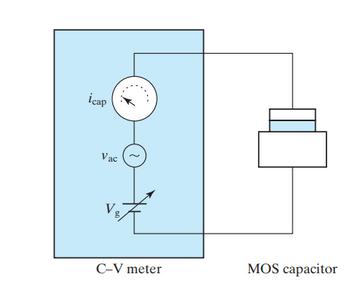
\includegraphics{MOS_C-V_measurement.png}
\end{center}
\begin{center}
    \emph{\hspace{2.5 cm}Setup for the C-V measurement\newline}
\end{center}
\par

\textbf{(a)} \textbf{Accumulation mode} \par
   In accumulation mode, the substrate charge is given by-
   \begin{center}
       $ Q_{acc} = -C_{ox}(V_{G}-V_{FB}) $
   \end{center}
  Going by the formula then, we have,
\begin{center}
    $ C = C_{ox} = \frac{\epsilon_{ox}}{t_{ox}}$
\end{center}
  Note that the capacitance under consideration is \emph{capacitance per unit area}. \par

\textbf{(b)} \textbf{Depletion mode} \par
    In depletion mode, the substrate charge is given by-
    \begin{center}
        $Q_{sub} = -qN_{A}W_{d}$
    \end{center}
    The gate voltage is given by-
    \begin{center}
        $V_{GS} = V_{FB} + \frac{qN_{A}W_{d}^{2}}{2\epsilon_{s}} + \frac{qN_{A}W_{d}}{C_{ox}}$
    \end{center}
    Thus, we obtain-
    \begin{center}
        $\frac{1}{C} = \frac{1}{C_{ox}} + \frac{W_{d}}{\epsilon_{s}} = \frac{1}{C_{ox}} + \frac{1}{C_{dep}}$
    \end{center}
   A bit of algebraic manipulation yields-
   \begin{center}
       $\frac{1}{C} = \sqrt{\frac{1}{C_{ox}^{2}} + \frac{2(V_{GS}-V_{FB})}{q\epsilon_{s}N_{A}}}$
   \end{center}
   
\textbf{(c)} \textbf{Inversion mode} \par
    In inversion mode, as we have seen earlier, the inversion charge is slow to change in a MOS capacitor. So, it is only under the influence of a low-frequency signal that the inversion charge layer can oscillate with time. In such a case, the capacitance of the system will be equal to the oxide capacitance (since $Q_{IN} = -C_{ox}(V_{GS}-V_{T})$). At high-frequency, the inversion charge remains constant whereas the charge inside the depletion region oscillates instead. In this case, the capacitance is given by-
    \begin{center}
        $C = -\frac{dQ_{dep}}{dV_{GS}}$
    \end{center}
    The capacitance in this case is the same as the depletion-mode capacitance at $V_{GS} = V_{T}$ (since we know that the depletion width is constant beyond $V_{T}$). \par
    
The following graph sums up the MOS C-V characteristics in different modes of operation: 

\par
\begin{center}
    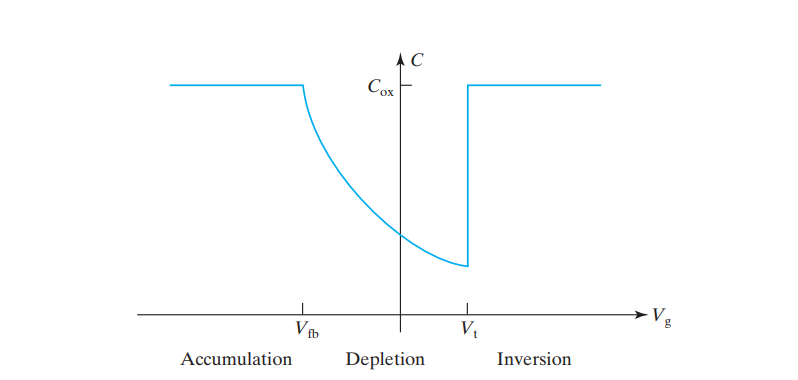
\includegraphics{MOS_C-V_characteristics.png}
\end{center}
\begin{center}
    \emph{\hspace{2.5 cm}Ideal MOS C-V characteristics\newline}
\end{center}
\par

The graph obviously depicts an ideal MOS capacitor. Practically, the graph is more complicated since many more factors have to be taken into account.

\par
\begin{center}
    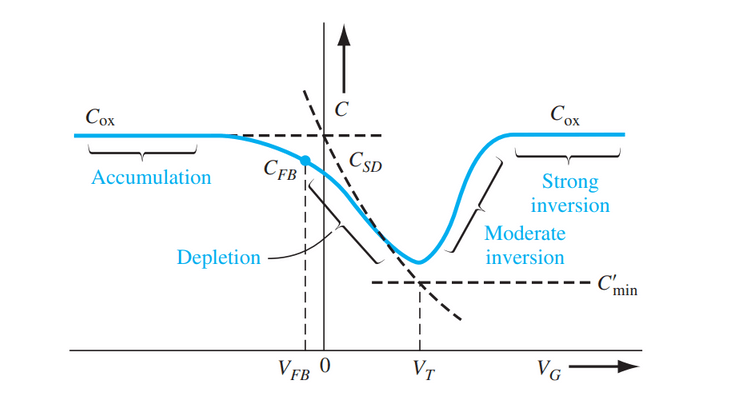
\includegraphics{MOS_C-V_char.png}
\end{center}
\begin{center}
    \emph{\hspace{2.5 cm}Experimental MOS C-V characteristics\newline}
\end{center}
\par

\href{https://upload.wikimedia.org/wikipedia/commons/7/78/Illustration_of_C-V_measurement.gif}{Here} is a highly instructive gif from Wikipedia depicting experimental variation of MOS capacitor with gate voltage against varying oxide thickness.

\subsection{MOSFET transistor}

According to the definition, a \href{https://en.wikipedia.org/wiki/Transistor}{transistor} is a semiconductor device capable of amplifying or switching electrical signals and power. In this light, the MOS capacitor clearly provides us an opportunity to create a transistor since we can turn on or off a current (which is attributable to the inversion charge), by simply modulating the gate voltage, $V_{GS}$. \newline

\par
\begin{center}
    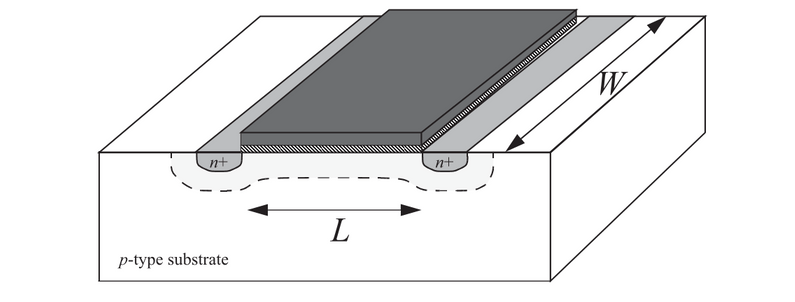
\includegraphics{MOSFET_1 (1).png}
\end{center}
\begin{center}
    \emph{\hspace{3 cm}Layout of a MOSFET\newline}
\end{center}
\par

\par
\begin{center}
    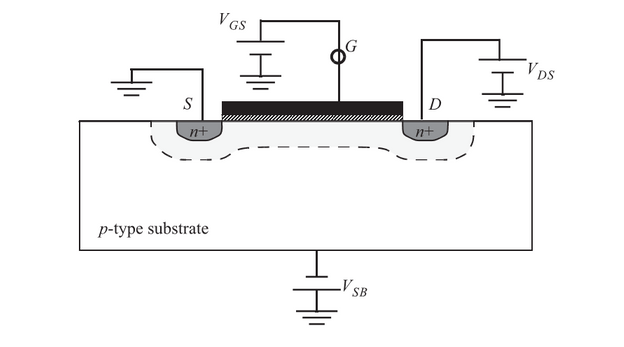
\includegraphics{MOSFET.png}
\end{center}
\begin{center}
    \emph{\hspace{3 cm}MOSFET structure\newline}
\end{center}
\par

Some of the basic differences between a MOS capacitor and a MOSFET are that while the MOS capacitor has no external source of minority carriers, the MOSFET has 'source' and 'drain' $n^{+}$ regions, which readily supply electrons. Thus, the MOSFET operates much faster in the inversion mode as compared to the MOS capacitor. Another important difference is the presence of an additional voltage source $V_{SB}$, which allows us to change the source-bulk voltage independent of the drain voltage or the gate voltage. This extra source is used to modulate the width of the depletion region and hence, the threshold voltage $V_{T}$. \par

The MOSFET I-V characteristics are derived by the Gradual Channel Approximation (GCA). The GCA states that as compared to the voltage variation along the y-axis (the direction perpendicular to the gate in the shown figure), the voltage variation along the x-axis (the direction from the sourcse to the gate) is quite slower. The inversion charge density acts like a sheet of charge along the x-axis and is also known as 'channel'. In a MOSFET, what happens physically is that on application of a drain voltage, $V_{DS}$ (while keeping $V_{GS} > V_{T}$), the electrons in the channel move from the source to the drain by drift processes (since the voltage changes very slowly along the channel, it also implies that the electron density also changes very slowly - hence the diffusion component can be ignored). The problem of current conduction through the channel can be broken up into two parts - an electrostatic one where inversion and depletion charges are accumulated along the x-direction and a dynamic one where $V_{DS}$ facilitates transport of electrons through channel. \newline

\par
\begin{center}
    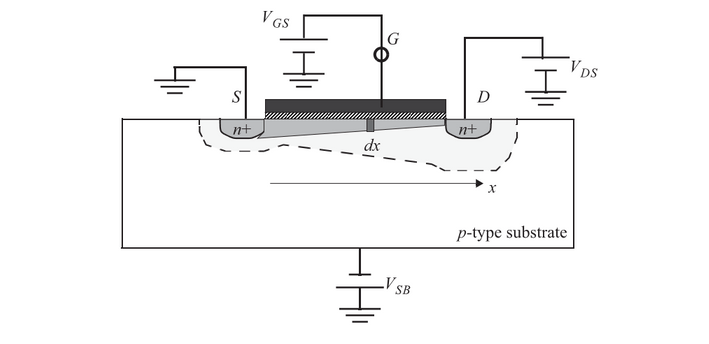
\includegraphics{MOSFET_2.png}
\end{center}
\par

The inversion charge distribution in the channel is such that the surface charge (w.r.t the oxide capacitance) can be expressed as $Q_{IN}(x)$ = n(x)$\Delta y$, where the volume charge density behaves as a kind of \href{https://en.wikipedia.org/wiki/Dirac_delta_function}{Dirac delta function}. In the light of this argument, consider an elemental strip along the y-axis as shown in the above figure. The resistance of the , dR, is given by-
\begin{center}
    $dR = -\frac{dx}{\mu_{n}Q_{IN}(x)W}$
\end{center}
where $W$ is the width of the channel, as shown in the structure of the MOSFET and $\mu_{n}$ is the mobility of electrons. The total channel charge, $Q_{S}(x)$ is given as $Q_{D}(x) + Q_{IN}(x)$. As per the voltage equations, 
\begin{center}
    $ V_{GS} = V_{FB} - \frac{Q_{S}(x)}{C_{ox}} + \phi_{s}(x) $
\end{center}
The term for $\phi_{s}$ now varies with position since there is an additional voltage drop in the channel now from drain to source due to the presence of $V_{DS}$ which drives the current. This implies,
\begin{center}
    $\phi_{s}(x) = 2\phi_{B} + V(x)$
\end{center}
Therefore, 
\begin{center}
    $ Q_{D}(x) = -\sqrt{2\epsilon_{s}qN_{A}(2\phi_{B}+V(x))}$
\end{center}
Applying Ohm's Law to the differential strip under consideration,
\begin{center}
    $ dV = I_{D}dR$
\end{center}
\begin{center}
    $I_{D}dx = -Q_{IN}(x)\mu_{n}WdV(x)$
\end{center}
On integrating,
\begin{center}
    $I_{D} = \frac{\mu_{n}C_{ox}W}{L}([V_{GS}-V_{T}-\frac{V_{DS}}{2}]V_{DS} -  \frac{2}{3}\frac{\sqrt{2\epsilon_{s}qN_{A}}}{C_{ox}}[(2\phi_{B}+V_{DS})^{3/2}-(2\phi_{B})^{3/2}])$
\end{center}

The term $\frac{\sqrt{2\epsilon_{s}qN_{A}}}{C_{ox}}$ is very small as compared to the other values and can practically be ignored without much loss of accuracy. The I-V characteristic then comes down to-
\begin{center}
    $I_{D} = \frac{\mu_{n}C_{ox}W}{L}([V_{GS}-V_{T}-\frac{V_{DS}}{2}]V_{DS})$
\end{center}
When the drain voltage is much smaller than $V_{GS}-V_{T}$, the I-V relation becomes linear-
\begin{center}
    $I_{D} = \frac{\mu_{n}C_{ox}W}{L}([V_{GS}-V_{T}]V_{DS}) $
\end{center}
This represents the linear mode of operation of a transistor and the channel effectively behaves as an ohmic resistor. At moderate values of $V_{DS}$, we cannot neglect its value in the I-V relation and have to use the exact relation itself. At still higher values of drain voltages, we encounter the situation of what is known as the 'saturation' region of operation. 

\subsubsection{Saturation mode}
As the gate voltage increases, at one point of time, it exceeds $V_{GS}-V_{T}$. In such a case, the inversion region in the vicinity of drain no longer exists and the channel is broken at that point. This point is known as \emph{pinch-off} mode of operation. At still higher drain voltages, the channel ends at some point close to the drain, but is not extended all the way to it as shown: \newline

\par
\begin{center}
    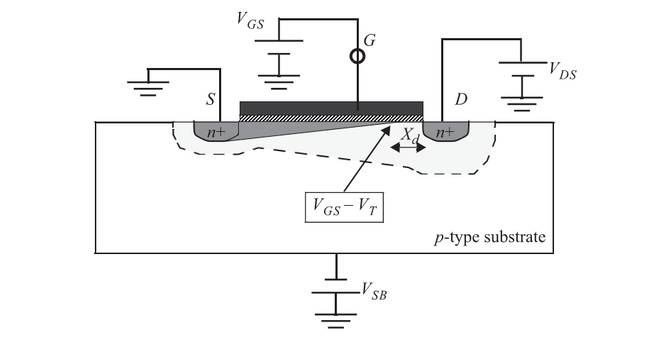
\includegraphics{MOSFET_3.png}
\end{center}
\begin{center}
    \emph{\hspace{2.5 cm}Pinch-off mode of operation\newline}
\end{center}
\par

In saturation mode, the inversion region no longer exists after the pinch-off point. Despite this, it does not prevent the carriers from conducting current in this region. The conduction in this region happens through the depletion region surrounding the conductive channel and drain and source regions. The resistance of this region is much higher than the channel and is quite similar to that of silicon (since there are very few carriers in the depletion region). Hence, most of the drain voltage drops across this region as compared to the highly conductive channel. Now, the distance of the drain from the pinch-off point is proportional to the drain voltage. So, the resistance offered by this region is thus, proportional to the drain voltage - which implies that the saturation current is \emph{independent} of the drain voltage, as observed experimentally. The saturation current is given by the value of drain current at the onset of saturation, i.e. when $V_{DS} = V_{GS}-V_{T}$. 
\begin{center}
    $I_{D,sat} = \frac{\mu_{n}C_{ox}W}{2L}(V_{GS}-V_{T})^{2}$
\end{center}
At saturation mode, GCA no longer holds true. However, the basic equation governing I-V characteristics remain unchanged and they can be solved in the same manner as we followed while deriving I-V characteristics for the MOSFET (for more clarity on this, refer to Problem 3(f)).  \par

The I-V characteristics of the MOSFET are summed up by this graph- \newline

\par
\begin{center}
    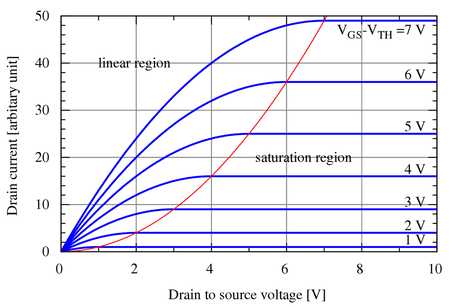
\includegraphics{MOSFET_I-V (2).png}
\end{center}
\begin{center}
    \emph{\hspace{2.5 cm}MOSFET I-V characteristics\newline}
\end{center}
\par

\section{Selected Problems}

\subsection{Problem 1}
A p-type semiconductor sample with acceptor concentration $N_{A}$, and length L, illustrated below, has ohmic contacts at both its ends. A light source generates $M_{A}$ electron-hole pairs/$cm^{2}$-s in the plane at x = $X_{A}$,i.e. $g_{L}(x) = M_{A}\delta (X_{A})$. Assume low-level injection and quasi-neutrality everywhere in the bar. 

\par
\begin{center}
    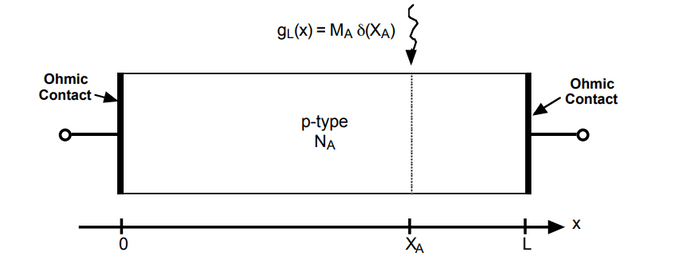
\includegraphics{problem_1_1.png}
\end{center}
\par

The general equation governing the excess minority carriers in a uniformly doped material is 
\begin{center}
    $ \frac{d^{2}n^{'}(x)}{dx^{2}}$ - $\frac{n^{'}(x)}{L_{e}^{2}} $ = $-\frac{1}{D_{e}}g_{L}(x)$
\end{center}

(a) What boundary condition is imposed on the excess minority carriers $n^{'}$ at x = 0 and x = L ? \par

(b) We now make the assumption that the minority carrier lifetime is very long, which simplifies the general equation to:
\begin{center}
    $ \frac{d^{2}n^{'}(x)}{dx^{2}} \approx -\frac{1}{D_{e}}g_{L}(x)$
\end{center}
What quantitative restriction is placed on the minority carrier lifetime, $\tau_{e}$, for this assumption to be valid ? \par

(c) Using the long-lifetime approximation in part (b), determine two constraints(i.e. boundary conditions) on the excess minority carriers at x = $X_{A}$, i.e. relating $n^{'}(X_{A^{-}})$ to $n^{'}(X_{A^{+}})$. \par

(d) Sketch the excess minority carrier concentration, $n^{'}(x)$ and the minority carrier diffusion current, $J_{e,diff}(x)$ everywhere inside the semiconductor. \par

(e) A second light source is added illuminating a single spot along the semiconductor at x = $X_{B}$, where $X_{B} > X_{A}$, and generating electron-hole pairs at a rate $M_{B}$, so that $g_{L}(x)$ is now 
\begin{center}
    $ g_{L}(x) = M_{A}\delta (X_{A}) $ + $ M_{B}\delta (X_{B}) $
\end{center}
Find $n^{'}(x)$ and $J_{e,diff}(x)$ under this new illumination condition. \par

\hspace{12 cm}[Courtesy : MIT OCW]

\href{https://drive.google.com/file/d/1gS-qn-ki6J5MHo3JBRmUMPuXIGdvap_n/view?usp=sharing}{Solution}

\subsection{Problem 2}
Consider the silicon diode pictured below. It is 4$\mu m$ long, with ohmic contacts at each end, and it is uniform p-type with $N_{A}$ = 1 x $10^{17}$ $cm^{-3}$ for 1 $\mu m$ on its far left end and uniform n-type with $N_{D}$ = 1 x $10^{17}$ $cm^{-3}$ on its far right end. In between these two uniformly doped regions, the net concentration, $N_{d}(x)-N_{a}(x)$, slowly grades linearly over a distance of 2 $\mu m$ from -1 x $10^{17}$ $cm^{-3}$ on the left to 1 x $10^{17}$ $cm^{-3}$ on the right, as shown in the lower figure. 

\par
\begin{center}
    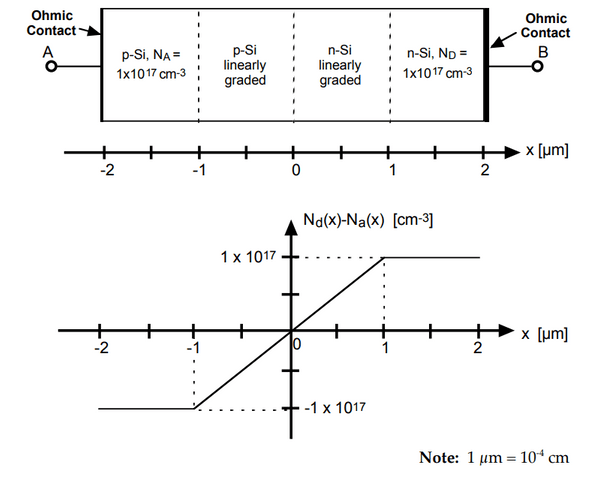
\includegraphics{problem_2_1.png}
\end{center}
\par

(a) In thermal equilibrium, what is the electrostatic potential, $\phi (x)$, in the left-hand quasi-neutral region at x = -1.5 $\mu m$, and what is the electrostatic potential, $\phi (x)$, in the right-hand quasi-neutral region at x = +1.5 $\mu m$, and what is the built-in potential step, $\Delta \phi _{b}$, seen transiting from x = -1.5 $\mu m$ to x = +1.5 $\mu m$ ? \par

(b) For the rest of this problem, a bias voltage, $V_{AB}$, is applied to this diode resulting in a total depletion region width of 1 $\mu m$, and $x_{N}$ =$|x_{P}|$ = 0.5 $\mu m$. Sketch and label the net charge density, $\rho (x)$ and the electric field, E(x), for -2$\mu m < x < 2\mu m$. \par

(c) What is the change in potential, $\Delta \phi$, transiting the depletion region when the bias is the same as in Part b, i.e. what is $\phi$(0.5 $\mu m$) – $\phi$(-0.5 $\mu m$) ? \par

(d) What is the change in potential, $\Delta \phi$, in transiting the quasi-neutral n-type graded region between x = 0.5 $\mu m$ and x = 1.0 $\mu m$, i.e. what is $\phi$(1.0 $\mu m$) – $\phi $(0.5 $\mu m$) ? \par

(e) What is the applied bias voltage, $V_{AB}$ ? \par

\hspace{11 cm} [Courtesy : MIT OCW]

\href{https://drive.google.com/file/d/19M9PUuE1QOvwd1e1w2vkUlPLHjnA2qOI/view?usp=sharing}{Solution}

\subsection{Problem 3}

The $I_{D}-V_{DS}$ plot for an ideal n-channel MOSFET is shown below. The substrate bias, $V_{BS}$, is 0 V, the saturation current, $I_{Dsat}$, is 10 mA, and the saturation voltage, $V_{DS,sat}$,is 5 V. For this device $t_{ox}$ = 10 nm, $\epsilon_{ox}$ = 3.5 x $10^{-13}$ F/cm, W = 50 $\mu$m, and L=10 $\mu$m. 

\par
\begin{center}
    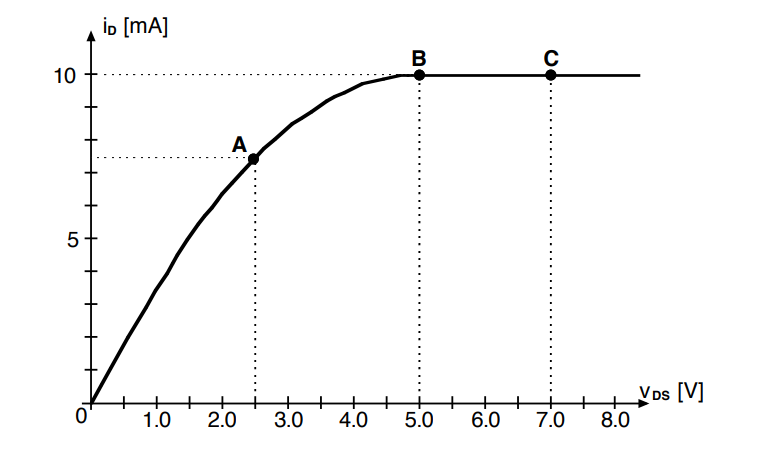
\includegraphics{MOSFET_IV.png}
\end{center}
\par

(a) Given that $V_{T}$ = 1 V, what is the gate voltage $V_{GS}$ that must be applied to obtain the characteristic shown above? \par

(b) What is the slope, $\frac{dI_{D}}{dV_{DS}}$ of the characteristic at $V_{DS}$ = 0 V ? Make sure you provide a formula as well as a value so that your answer is independent of the correctness of your Part (a). \par

(c) Assuming that $V_{T}$ is independent of position in the channel, calculate the inversion layer sheet charge density, $q_{N}^{*}(y)$ corresponding to Bias Point A (i) adjacent to the source (the source end, y = 0) and (ii) adjacent to the drain (drain end, y = L). \par

(d)  Calculate the electron drift velocity, $s_{e-Drift}$, at the (i) source end and (ii) drain end of the channel at Bias Point A. \par

(e) The transistor enters saturation at Bias Point B and simple theory suggests that the drain-end charge has become 0 while the drain-end velocity is infinite, so that the $I_{Dsat}$ can flow in that part. Now, assuming instead that the electrons at the drain end move at their saturation velocity, $s_{sat} = 10^{7}$ cm/s, what is the channel charge density that must exist there to support the $I_{Dsat}$ ? \par

(f)  Assuming $V_{CS}$(y) is the voltage that a hypothetical voltmeter would measure between the inversion layer at position y along the channel and the source. Derive an expression that could be solved for $V_{CS}$(L/2), i.e. at distance L/2 from the source in a device biased at Bias Point C, in terms of the transistor parameters and $I_{Dsat}$. \par

\hspace{12 cm}[Courtesy : MIT OCW]

\href{https://drive.google.com/file/d/13Ysh57hD2lzxWlqpqbpQ9mMU5Yj2v9dc/view?usp=sharing}{Solution}

\subsection{Problem 4}

Consider the $n^{+}-p$ diode shown below in thermal equilibrium. The $n^{+}$ doping in Region 1 is high enough that it is degenerate, with $\phi_{n^{+}}$ = 0.55 V. Assume that the depletion region on the $n^{+}$ side of the junction is negligibly small so that you may also assume negligible change in potential across it. Note too that Region 2, the $p^{-}$ Si region, is very lightly doped (i.e. $N_{A2} < 10^{13}$ $cm^{-3}$). Finally, L = 0.2 $\mu$m (= 2 x $10^{-5}$ cm). [$\phi_{n^{+}}$ refers to the energy difference between intrinsic band and Fermi level in Region 1]  \par

\par
\begin{center}
    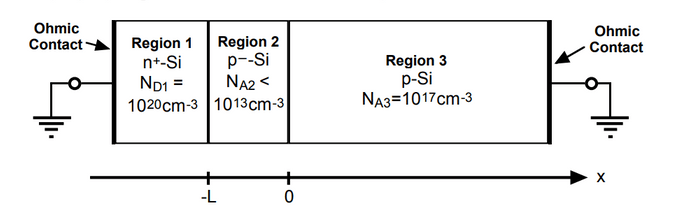
\includegraphics{Problem_4.png}
\end{center}
\par

(a) Calculate $\Delta\phi_{13}$, the built-in potential difference between the QNR (quasi-neutral region) in Region 1 (i.e. where x $<<$ -L) and the QNR in Region 3 (where x $>>$ 0). \par

(b) Sketch and label $\rho(x)$, the net charge density, and E(x), the electric field, in the structure. You should label the depletion region width in Region 3 as $x_{D}$ (you are not expect to find a value for $x_{D}$). You may assume that the width of the depletion region in Region 1 is negligibly small (so that there is essentially an impulse of charge at x = -L). \par

(c) Set up an equation with $x_{D}$, the width of the depletion layer in Region 3, being the only unknown, that you could use to find $x_{D}$.  \par

(d) Give an expression for $C^{*}_{dp}$, the depletion capacitance per unit area of this device at zero bias, V = 0 volts. $x_{D}$ can appear as a parameter in your expression.  \par

\hspace{12 cm}[Courtesy : MIT OCW]

\href{https://drive.google.com/file/d/1WXVlVUPrEufr3gocBx2el-wyhII5PUq3/view?usp=sharing}{Solution}

\subsection{Problem 5}

Alice is a process engineer experimenting with a new high-permittivity dielectric material with a dielectric constant, $\epsilon_{hi}$, that is 5 times as large as the dielectric constant of $SiO_{2}$, i.e. $\epsilon_{hi} = \epsilon_{ox}$. She chooses to test the material by fabricating p-MOS capacitors on n-type silicon, and to use a metal for the gate and contact for which $\phi_{m}$ = - 0.5 $\phi_{n}$. Her structure is illustrated below; it also includes an adjacent $p^{+}$ region shorted to the substrate (not shown in the figure) to supply holes when an inversion layer is formed.

\par
\begin{center}
    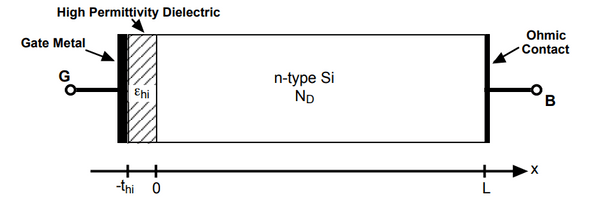
\includegraphics{Problem_5.png}
\end{center}
\par

(a) Sketch the electrostatic potential, $\phi (x)$, through the device from G to B (i.e. starting in the gate metal and going into the ohmic contact metal) in flatband when $V_{GB}$ = $V_{FB}$. Label all relevant features on your plot, including values for $\phi (0)$, depletion region width, and potential drop across the oxide. Finally, derive an expression for the flatband voltage, $V_{FB}$.  \par

(b)  At flatband, i.e. with $V_{GB}$ = $V_{FB}$, what are the electron and hole concentrations, n(x = $0^{+}$) and p(x = $0^{+}$), at the silicon-dielectric interface? \par

(c) Sketch the electrostatic potential, $\phi(x)$, and the charge distribution, $\rho (x)$, through the device from G to B at the onset of inversion, i.e. when $V_{GB} = V_{T}$. Label all relevant features on your plots, including values for $\phi (0)$, depletion region width, and potential drop across the oxide. Finally, derive an expression for the threshold voltage, $V_{T}$.  \par

(d) At the onset of inversion, i.e., when $V_{GB} = V_{T}$,what are the electron and hole concentrations, n(x = $0^{+}$) and p(x = $0^{+}$), at the silicon-dielectric interface?  \par

(e) A practical problem with depositing a dielectric other than $SiO_{2}$ directly on silicon is that new energy states and/or fixed sheet charge are introduced at the interface. Imagine that the latter occurs, and that there is a fixed positive sheet charge density, $\sigma_{i}$, at the interface. Assuming that this charge can be modeled as an impulse of charge of intensity $\sigma_{i}$ at x = 0, i.e. $\rho(x) = \sigma_{i} \delta(x)$, calculate the changes in the flatband voltage, $V_{FB}$, and in the threshold voltage, $V_{T}$, resulting from the presence of this charge.  \par

(f) To eliminate the interface charge, a very thin layer of silicon dioxide, $SiO_{2}$, can be grown on the silicon before the high permittivity dielectric is deposited, as illustrated in the figure below. How much is the gate dielectric capacitance, $C_{G}$, changed relative to its original value in Part (a) by the addition this $SiO_{2}$ layer if $t_{ox} = 0.2 t_{hi}$?  

\par
\begin{center}
    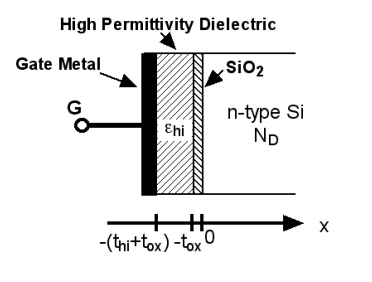
\includegraphics{Problem_5_1.png}
\end{center}
\par

\hspace{12 cm}[Courtesy : MIT OCW]

\href{https://drive.google.com/file/d/13iGpw3SyTD3zXcj59EY4Y-b9aaFxUMzM/view?usp=sharing}{Solution}

\section{Formula Sheet}
Keeping in view the difficulty in dealing with the large number of formulae involved in this project, here is a \href{https://drive.google.com/file/d/1jcVRobZqQsFGafdbbzfPG_H4w_CabpKo/view?usp=sharing}{formula sheet} compiled by me to serve as a quick reference.

\section{References}

1. Ben G. Streetman, Sanjay Kumar Banerjee. Solid State Electronic Devices, Pearson Publications, 2018.\newline \newline
2. Tak H. Ning, Yuan Taur. Fundamentals of Modern VLSI Devices, Cambridge   University Press, 2009. \newline \newline
3. Chenming Calvin Hu. Modern Semiconductor Devices for Integrated Circuits,
Pearson Publications, First Edition. \newline \newline
4. Prof.Digbijoy N. Nath. NPTEL course-\href{https://www.youtube.com/playlist?list=PLgMDNELGJ1CaNcuuQv9xN07ZWkXE-wCGP}{Fundamentals of semiconductor devices}. IISc Bangalore. \newline \newline
5. Prof.Clifton Fonstad. \href{https://ocw.mit.edu/}{MIT OpenCourseWare} course - \href{https://ocw.mit.edu/courses/6-012-microelectronic-devices-and-circuits-fall-2009/}{Microelectronic Devices and Circuits}. \newline \newline
6. Prof.Ali Hajimiri. \href{https://chic.caltech.edu/links/}{CHIC, Caltech} \newline \newline
7. \href{https://en.wikipedia.org/wiki/Main_Page}{Wikipedia.org} \newline \newline
8. \href{http://hyperphysics.phy-astr.gsu.edu/hbase/index.html}{Hyperphysics} \newline \newline
9. \href{https://physics.stackexchange.com/}{Physics Stack Exchange} \newline \newline
10. \href{https://eng.libretexts.org/Bookshelves/Electrical_Engineering}{Electrical Engineering LibreTexts} \newline \newline

\end{document}